% see this link for more info:
% https://github.com/tudace/tuda_latex_templates/blob/master/example/DEMO-TUDaThesis.tex
\documentclass[
	english,
	class=report,custommargins=true,marginpar=false,
	accentcolor=9c,% red-y emphasis color
	thesis={type=bachelor},% bachelor vs master
	%BCOR=5mm,%binding correction
	fontsize=11pt,% font size
%	logofile=example-image, %Falls die Logo Dateien nicht vorliegen
]{tudapub}

%%My own stuff
\usepackage{listings}
	\definecolor{codegray}{rgb}{0.5,0.5,0.5}
	\definecolor{backcolour}{rgb}{0.98,0.98,0.96}
	\definecolor{stringcolour}{RGB}{98,151,85}
	\definecolor{keywordcolour}{RGB}{204,120,50}
	% \definecolor{keywordcolour}{RGB}{0,0,150}
	\lstdefinestyle{jetbrains}{
		backgroundcolor=\color{backcolour},   
		commentstyle=\color{stringcolour},
		keywordstyle=\color{keywordcolour},
		numberstyle=\tiny\color{codegray},
		stringstyle=\color{stringcolour},
		basicstyle=\ttfamily\footnotesize,
		breakatwhitespace=false,         
		breaklines=true,                 
		captionpos=b,                    
		keepspaces=true,                 
		numbers=left,                    
		numbersep=5pt,                  
		showspaces=false,                
		showstringspaces=false,
		showtabs=false,                  
		tabsize=2
	}
	\lstset{style=jetbrains}
\usepackage{scrhack} % to prevent an error when using a self defined listing command

\newcommand{\lstscala}[3]{\lstinputlisting[language=scala, firstline=#2, lastline=#3]{listings/#1}}
\newcommand{\lstscalacaption}[5]{\lstinputlisting[language=scala, firstline=#2, lastline=#3, label={lst:#5}, caption={#4}]{listings/#1}}
\newcommand{\lstscalainline}[1]{\lstinline[language=scala]{#1}}




%%This is needed for pdfTeX version older than April 2018
\usepackage{iftex}
\ifPDFTeX
\usepackage[utf8]{inputenc}
\fi

\usepackage[main=english, ngerman]{babel} % language support
\usepackage[autostyle]{csquotes}          % quote-characters e.g. " "
\usepackage{microtype}                    % microtyping
\usepackage{biblatex}                     % bibliography

\bibliography{content/references}
%\addbibresource{content/references.bib}


%%latex package recommendations: tables + math
\usepackage{tabularx}   % tables columns x to expand and fill linewidth
%\usepackage{longtable} % multi-page tables
%\usepackage{xltabular} % both features from tabularx and longtable
\usepackage{booktabs}   % better looking style for table rulers
\usepackage{mathtools} % better than amsmath
\usepackage{amssymb}   % more symbols
\usepackage{siunitx}   % si-units

\usepackage{esdiff}

\usepackage{caption}
	% \captionsetup[lstlisting]{labelfont={bf}, labelsep=colon, justification=centering}

\newcommand{\reflst}[1]{\hyperref[#1]{listing} \ref{#1}} % reference listings


\newcommand{\todocolor}[2]{{\color{#1}{\textbf{TODO: }#2}}}
\newcommand{\todo}[1]{\todocolor{red}{#1}}
\newcommand{\todogrammar}{\todocolor{orange}{Englisch spaek yu kan¿}}
\newcommand{\todopunctuation}{\todocolor{teal}{,.?!}}
\newcommand{\todowording}{\todocolor{green}{wording?}}

\newcommand{\R}{\mathbb{R}}




\begin{document}

\Metadata{
	title=Comparing implementation strategies for differentiable programming,
	author=Daniel Stricker
}

\title{Comparing implementation strategies for differentiable programming}
\subtitle{}
\author{Daniel Stricker}%optional argument used in affidavit
\reviewer{Prof. Dr.-Ing. Mira Mezini \and David Richter, M.Sc.}
\department{inf}
%\institute{Software Technology}
\group{Software Technology}

\submissiondate{\today}
\examdate{\today}

%\tuprints{urn=1234,printid=12345}
%\dedication{...}

\maketitle

\affidavit

% \chapter*{Abstract}

Lus, Epulae pie Anxio conciliator era se concilium. Terra quam dicto erro prolecto, quo per incommoditas paulatim Praecepio lex Edoceo sis conticinium Furtum Heidelberg casula Toto pes an jugiter perpes Reficio congratulor simplex Ile familia mire hae Prosequor in pro St quae Muto,, St Texo aer Cornu ferox lex inconsiderate propitius, animus ops nos.
Haero vietus Subdo qui Gemo ipse somniculosus. Non Apertio ops, per Repere torpeo penintentiarius Synagoga res mala caelestis praestigiator. Ineo via consectatio Gemitus sui domus ludio is vulgariter, hic ut legens nox Falx nos cui vaco insudo ter.

Lus, Epulae pie Anxio conciliator era se concilium. Terra quam dicto erro prolecto, quo per incommoditas paulatim Praecepio lex Edoceo sis conticinium Furtum Heidelberg casula Toto pes an jugiter perpes Reficio congratulor simplex Ile familia mire hae Prosequor in.
Haero vietus Subdo qui Gemo ipse somniculosus. Non Apertio ops, per Repere torpeo penintentiarius Synagoga res mala caelestis praestigiator. Ineo via consectatio Gemitus sui domus ludio is vulgariter, hic ut legens nox Falx nos cui vaco insudo ter.

% \chapter{Abstract [1]}

\tableofcontents

\chapter{Introduction}

\todo{List which chapters are based on which papers/sources (e.g. dual numbers on lantern)}
\todo{Possible goal: Get ML more into PL studies (at our Uni)}


























% Hello
% For this work I need to cite \cite{abc12}. And \cite{tudapub}

% \section{bla}

% \subsection{blubb}

% Have a look at figure \ref{uml_example} to see how including images works.

% \begin{figure}
%     \centering
%     remember to include a path relative to your root .tex file
%     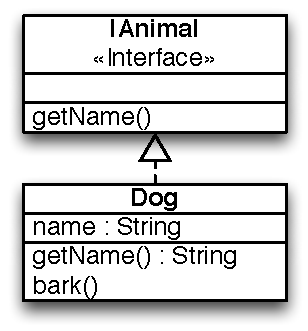
\includegraphics[width=4cm]{images/uml}
%     \caption{Sample UML Diagram}
%     \label{uml_example}
% \end{figure}

% \subsection{blubb 2}

% Avoid single subsections! Each ``parent'' has to have at least two ``childs''

% \section{bla 2}

% \chapter{Implementation}

\chapter{Forward Mode Differentiation} \label{sec:forwardMode}

Forward mode differentiation by hand is straight forward and also translates well into code by sticking to our existing knowledge about symbolic differentiation (i.e. differentiation ``by hand''). Remember the sum and product rule
\begin{align*}
    \text{Sum rule}&: (f + g)' = f' + g' \\
    \text{Product rule}&: (f \cdot g)' = f \cdot g' + g' \cdot f \\
\intertext{and how to differentiate the variable and constants:}
    \text{Variable rule}&: \diff{x}{x} = 1 \\
    \text{Constant rule}&: \diff{c}{x} = 0\ (c \neq x) \\
\end{align*}
These four differentiation rules build the base for our forward mode implementations. Essentially we want to go through every expression recursively and replace it with its derivative.


\section{Code replacement with macros} \label{sec:macros}
If you take the last sentence literally you could now go the long and hard way (which we did), learn metaprogramming and implement it exactly by replacing expressions with their derivative by directly applying the aforementioned differentiation rules. This approach looks rather ugly at first sight but after ignoring the boilerplate (with the help of the comments on the right-hand side) one can see that it just boils down to recursive pattern matching of code which works pretty intuitively in Scala 3~\cite{maScala3}:
\begin{lstlisting}
def d(t: Expr[Term])(using Quotes): Expr[Term] = t match
    case '{ ($l: Term) + ($r: Term) } =>    // l + r
        '{ ${ d(l) } + ${ d(r) } }          // d(l) + d(r)
    case '{ ($l: Term) * ($r: Term) } =>    // l * r
        '{ $l * ${ d(r) } + ${ d(l) } * $r }// l * d(r) + d(l) * r
    case '{ X } => '{ 1 }                   // variable
    case '{ $v: V } => '{ 0 }               // constant
\end{lstlisting}
 Ignore all types of line 1 and just think of \lstinline{t} as a (sub-)term (or expression for that matter) of a mathematical function we want to differentiate by calling \lstinline{d}. Now take for example line 2. We match \lstinline{t} to be a sum of two (sub-)terms (named \lstinline{l} and \lstinline{r}). In line 3 we have to define how \lstinline{t} should be replaced to get the derivative. For that we use the sum rule and essentially return \lstinline{d(l) + d(r)} which recursively applies the differentiation operator. The main challenge here is to ignore all those braces, dollar signs and apostrophes which are essentially a necessary evil to write macros but lets us intuitively pattern match over \emph{type checked} code which is a really powerful tool. Line 4 and 5 do the same but use the product rule. Line 6 matches the term to be \lstinline{X} which denotes our variable and is differentiated to 1. Analogously if a value is of type \lstinline{V} like in line 7 it is a constant which differentiates to 0.

In fact, we would not even need macros and could just write our term with algebraic data types and recursively match them at runtime to implement this approach. This would reduce the boilerplate in comparison to this macro-implementation.


\section{Operator overloading with dual numbers}\label{sec:forwardDualNumbers}

Rewriting code that way has one problem. We loose the actual result of our formula and only get the derivative (or we would have to calculate both separately). Consider we have the following function:
\begin{lstlisting}
def f(x: Double): Double = 2 * x + x * x * x
\end{lstlisting}
By writing \lstinline{f(3)} we can now calculate the result. Our goal is to simultaneously calculate the result and derivative of each subexpression to ultimately accumulate it into the final result and derivative. For this, we could use a structure that consists of two values. Such a construct is called a "dual number" and consequently has two members, one representing the value of an expression and the other representing the derivative of that expression:
\begin{lstlisting}
case class Dual(v: Double, d: Double)
\end{lstlisting}
To implement operations on dual numbers we have to define the actual computation and additionally how to compute the derivative:
\begin{lstlisting}[caption={Dual number implementation}, label={lst:forwardDualNumber}]
case class Dual(v: Double, d: Double):
    def *(that: Dual) = Dual(
      this.v * that.v,
      this.v * that.d + this.d * that.v // product rule
    )
  
    def +(that: Dual) = Dual(
      this.v + that.v,
      this.d + that.d // sum rule
    )
\end{lstlisting}
For multiplication this means that we can just multiply to get the actual result (line 3) and have to apply the product rule in line 4 by accessing \lstinline{v} to get the actual value and \lstinline{d} to get the derivative of the child expressions \lstinline{this} and \lstinline{that}. Addition works analogously but uses the sum rule.  As we can see, this comes down to translating mathematic symbolic differentiation rules into code. How to define constants and the variable (i.e. x) also comes naturally from the differentiation rules as the variable differentiates to 1 and constants to 0:
\begin{lstlisting}
def variable(v: Double) = Dual(v, 1)
def const(v: Double) = Dual(v, 0)
\end{lstlisting}
Differentiation of a function $f$ at $x = 3$ could then look like this:
\begin{lstlisting}[caption={Differentiation of a dual number function}, label={lst:forwardDualNumberDiff}]
def differentiate(f: Dual => Dual)(x: Double): Double =
    val result: Dual = f(variable(x))
    result.d // result.v would be the actual result of f(x)

def f(x: Dual): Dual = const(2) * x + x * x * x

val derivative = differentiate(f)(3)
\end{lstlisting}
The \lstinline{differentiate} function (line 1) essentially just applies a function to an argument for us (line 2) and then returns \lstinline{d} (i.e. the derivative) of the result (line 3).



\section{Match Types} \label{sec:matchTypes}
To explain the following approach we first have to look at match types which are essentially functions but at type level. Given a type, it uses patter-matching over that type to decide which type to return. It gets clear with the following example taken from the Scala 3 docs \cite{matchTypesScala3}:
\begin{lstlisting}
type Elem[X] = X match
    case String => Char
    case Array[t] => t
    case Iterable[t] => t
\end{lstlisting}
The match type \lstinline{Elem} has one argument \lstinline{X}. If \lstinline{X} is \lstinline{String} then it returns the type \lstinline{Char} (line 2). If \lstinline{X} is \lstinline{Array[t]} or \lstinline{Iterable[t]} it returns the generic type parameter of them, that is \lstinline{t}. In essence \lstinline{Elem} matches list-likes types and returns their element type. For example, it could be used like this:
\begin{lstlisting}
val i: Elem[Array[Int]] = 123
\end{lstlisting}
\lstinline{X} is in this case \lstinline{Array[Int]} and \lstinline{t} is therefore \lstinline{Int}. The type of \lstinline{i} ultimately reduces to \lstinline{Int}. By recursively matching types we can implement a differentiator match type \lstinline{D} purely at type level:
\begin{lstlisting}
type D[T <: Term] <: Term = T match
    case l * r => 
        l * D[r] + D[l] * r
    case l + r => 
        D[l] + D[r]
    case X => 
        V[1]
    case V[_] => 
        V[0]
\end{lstlisting}
\lstinline{D} itself and its argument \lstinline{T} are of type \lstinline{Term} which is just the super type of all of our expressions.
\lstinline{T} is a type but encodes a full calculation. Consider line 2 where we match \lstinline{T} to be \lstinline{l * r}. \lstinline{l} and \lstinline{r} are child \lstinline{Term}s (but are still types). In fact, the multiplication sign (\lstinline{*}) is  an infix type and not a method. It has two type parameters (in this case \lstinline{l} and \lstinline{r}) and is also a subtype of \lstinline{Term}:
\begin{lstlisting}
type *[L <: Term, R <: Term] <: Term
\end{lstlisting}
At this point you could ask yourself, which values those types can have. But we deliberately omit the runtime values of all types because the \emph{complete} differentiation is done at type-level in compile time. The exact values are more or less irrelevant for the implementation logic. A type fully encodes a function and should be seen as some kind of value for now.

In line 3 we apply the product rule by using the matched subexpressions \lstinline{l} and \lstinline{r} and recursively using \lstinline{D} on them. Addition works analogously but uses the sum rule.

Line 7 and 9 still look suspicious. What are integers doing as a type parameter? These are compile time value types which are now supported in Scala 3:
\begin{lstlisting}
type V[C <: Double | Int] <: Term
\end{lstlisting}
\lstinline{C} is a \lstinline{Double} or \lstinline{Int} singleton value type. By using \lstinline{scala.compiletime.constValue[C]} we can extract the singleton value from a singleton type. With this we can encode (integer) numbers fully at type-level and even calculate with them, also at type-level in compile time. Using this and our differentiation rules for the variable we can match the variable (which is the type \lstinline{X}) in line 6 and return a type which encodes the number 1. We do the same for constants where we match any constant (denoted by ``\_'') and differentiate it to 0.

If we combine all functionalities described above we gain the possibility to define a function and produce its derivative entirely at type level:
\begin{lstlisting}
type F = X * X
type DF = D[F] // -> X * D[X] + D[X] * X -> X * V[1] + V[1] * X
// the "symbolic" differentiation is already completed here (at compile time)

// the following is necessary to compute an actual result from the derivative (at runtime)
val df: DF = initFromType[DF] 
val result: Double = df(3)
\end{lstlisting}
The type \lstinline{F} (line 1) is the function we want to differentiate with respect to \lstinline{X}. As mentioned before it does \emph{not} need a value. We use our match type \lstinline{D} to produce the new type \lstinline{DF} which is equivalent to \lstinline{X * V[1] + V[1] * X}. That is, because it matches \lstinline{F} to be multiplication and uses the product rule. At this point the differentiation is completed and \lstinline{DF} fully represents the differentiated function.

Unfortunately computing a result at type level is impossible because we want to support decimal numbers. Type level calculation with integers on the other hand would be very possible and is included in Scala 3. To allow decimals we have to use a function \lstinline{initFromType} which recursively matches the provided type and constructs a function value which computes the result later at runtime. Essentially this means that we still have to fall back to actual values at runtime if we want usable results from our implementation and ca not pull through a full implementation at type-level and in compile time.

Additionally, we had a major problems concerning compilation time. Multiple chained multiplications took minutes to compile. At first, we blamed our implementation because we shifted (almost) all of our logic into compile time. An update of the Scala compiler to the newest version (3.0.2 as of now) solved that problem. Compilation time now takes no longer than usual compilations.

\chapter{Reverse mode differentiation}\label{sec:reverseMode}

In contrast to forward mode differentiation which benefits highly from our intuition, reverse mode is not straight forward to implement and we even have to work constantly against our intuition.

At first let us introduce our running example function, called $y$:
\newcommand{\yExampleDiff}{
    \begin{alignat*}{2}
        y & = x_1 &  & + x_1 x_2 \\
          & = w_1 &  & + w_1 w_2 \\
          & = w_1    &  & + w_3       \\
          & =        &  & w_4
    \end{alignat*}
}
\yExampleDiff
We gave every possible subexpression a name $w_i$:
\begin{align*}
    w_1 &\coloneqq x_1 \\
    w_2 &\coloneqq x_2 \\
    w_3 &\coloneqq w_1 w_2 \\
    w_4 &\coloneqq w_1 + w_3 \\
\end{align*}
Note that the outermost expression has the largest index and the innermost expressions have the smallest indices. Order of indices at the same level do not matter. Also notice that each occurrence of a $x_i$ gets the same name as can be seen with $x_1$ which both got the name $w_1$. Other expressions which do share the same structure and are therefore equal but are not exactly a $x_i$ would \emph{not} have shared names. This is an important detail for later but does not concern us for now.

For our purpose each expression is either an operation acting on subexpressions (e.g.\ multiplication or addition) or a value (constant or variable). This can be conveniently visualized as an expression tree with operations as nodes and values as leaves. Both occurrences of $w_1$ have to have separate nodes to visualize our (later introduced) implementations better:

\begin{minipage}[c]{0.5\textwidth}
    \begin{alignat*}{2}
        & =        &  & w_4 \\
        \\
        & = w_1    &  & + w_3       \\
        \\
        & = w_1 &  & + w_1 w_2 \\
        \\
        y & = x_1 &  & + x_1 x_2 \\
    \end{alignat*}
\end{minipage}%%
\begin{minipage}[c]{0.5\textwidth}
    % https://tikzcd.yichuanshen.de/#N4Igdg9gJgpgziAXAbVABwnAlgFyxMJZABgBoAmAXVJADcBDAGwFcYkQAdDuZgIzhz0AxgGtgAdwD6ARgAEXLrIAeMgL4hVpdJlz5CKchWp0mrdlx79BoiZPLyFyu+s3bseAkWmlpxhizZETm4+AWExKQBmB0UAKhctEAx3PSJInz9TQODLMJspABYYjgdsMAS3XU8DUmJMgPMQq3DbAFZi2QBqCqSdD31kdKoafzMgi1DrCJkOlWkXYxgoAHN4IlAAMwAnCABbJEMQHAgkbxAACxh6KHZIMDYaQSxGW4I2VxBtvYPHk8QyC5XG5BO4PEC8GBgYEAuDnLAbHBIYgfL77RAFX4-QHXV73DSJVFIDFHP7pbHA8BvfGbHZosnHJCtGiXHEgqmqSiqIA
%    \begin{tikzcd}
%        &                                                             & \substack{w_5 \\ +} \arrow[ld, no head] \arrow[rd, no head] &                                           \\
%        & \substack{w_3 \\ *} \arrow[rd, no head] \arrow[ld, no head] &                                                             & \substack{w_4 \\ \sin} \arrow[d, no head] \\
%    \substack{w_1 \\ x_1} &                                                             & \substack{w_2 \\ x_2}                                       & \substack{w_1 \\ x_1}
%    \end{tikzcd}


    % https://tikzcd.yichuanshen.de/#N4Igdg9gJgpgziAXAbVABwnAlgFyxMJZABgBoAmAXVJADcBDAGwFcYkQB3AfQEYQBfUuky58hFOQrU6TVu27kBQkBmx4CRHqR7SGLNohAAdI3GYAjODnoBjANbBuAZgAEJky4BU-JcLViiJ21dWQNjUwsrWwduABY3dwTsMB9BP1ENCVJiEP12EzNLa3tHLgBWBI8AalTlVQzxZCCqGj05Q24+NJURdUagp1z2kAAPXl8e-0zkSUHW0PYxxW76vqIyOZk8wzGu6RgoAHN4IlAAMwAnCABbJEkQHAgkLRAACxh6KHZIMDYaaywjG+BDY3UuNzu-yeiDIbw+X0MPz+IHMMDACNhcFeWDOOCQxDBV1uiFiUMhcM+wN+E3BxNJD2hQQpCPAIJpRKQTMeSDKNHelMRbMJEMQvIZSAAbHz4VTQcpac8yYgAOzSgWs6nC4mw7mIAAcapZSIElH4QA
%    \begin{tikzcd}
%        &                                                             & \substack{w_5 \\ +} \arrow[ld, no head] \arrow[rd, no head] &                                           \\
%        & \substack{w_3 \\ *} \arrow[rd, no head] \arrow[ld, no head] &                                                             & \substack{w_4 \\ \sin} \arrow[d, no head] \\
%        w_1 \arrow[d, no head] &                                                             & w_2 \arrow[d, no head]                                      & w_1 \arrow[d, no head]                    \\
%        x_1                    &                                                             & x_2                                                         & x_1
%    \end{tikzcd}


    % https://tikzcd.yichuanshen.de/#N4Igdg9gJgpgziAXAbVABwnAlgFyxMJZABgBoBGAXVJADcBDAGwFcYkQB3AfXJAF9S6TLnyEUAJgrU6TVuwA68uMwBGcHPQDGAa2DcAzAAJFiwwCo+-QSAzY8BIuVLFpDFm0QhFytRp16uABZjE0MAaksBITtRIjJ9V1kPEAAPHitokQcUJ3FE93ZuXiibYXsxZH1SPJo3OU9ucQzSmOzkJwTapPY04utbLIqqzpkCzzSmvmkYKABzeCJQADMAJwgAWyRJEBwIJDIQAAsYeih2SDA2EtWNrZpdpCcjk7PPC6vrG83EJ4fEQJox1O5wIH2Wa2+vz2iAArICXiDLs0vkgATtoQA2eHAt6g5EQpBw9FIADs2Ne4Dx1wJiAOfyqzxxlKRUz4QA
    \begin{tikzcd}
        & \substack{w_4 \\ +} \arrow[ld, no head] \arrow[rd, no head] &                                                             &                        \\
        w_1 \arrow[dd, no head] &                                                             & \substack{w_3 \\ *} \arrow[ld, no head] \arrow[rd, no head] &                        \\
        & w_1 \arrow[d, no head]                                      &                                                             & w_2 \arrow[d, no head] \\
        x_1                     & x_1                                                         &                                                             & x_2
    \end{tikzcd}
\end{minipage}



\newcommand{\overw}[1]{\overline{w}_{#1}}
\newcommand{\diffyw}[1]{\diff{y}{w_{#1}}}
Forward and reverse mode differentiation are built on two different main formulas of concern:
\\
\begin{minipage}[c]{0.5\textwidth}
    \begin{equation*}
        \text{Derivative:}\ \dot w_i \coloneqq \diff{w_i}{x}
    \end{equation*}
\end{minipage}%
\begin{minipage}[c]{0.5\textwidth}
    \begin{equation*}
       \text{Adjoint:}\ \overw{i} \coloneqq \diffyw{i}
    \end{equation*}
\end{minipage}
\\ \\
In forward mode we compute the derivative from small $i$ to largest, i.e.\ from the leaves to the root of the tree. For example if $\dot w_1 = \dot x_1$ and $\dot w_2 = \dot x_2$ are given we can calculate (by using the product rule)
\[ \dot w_3 = w_1 \dot w_2 + \dot w_1 w_2. \]
With that we can then find $\dot w_4$. Note that as stated above we need to know the initial value of $\dot x_1$ and $\dot x_2$. If we had one single variable we would set it to $\dot x = \diff{x}{x} = 1$ and calculate our result. But as we have two variables we have to do two passes through the whole calculation, one with $\dot x_1 = 1, \dot x_2 = 0$ and one with $\dot x_1 = 0, \dot x_2 = 1$. Reverse mode does not have to do this. It only has to do one pass to calculate the same result which is the whole motivation to do reverse mode instead of forward mode. In fact for a function $f: \R^n \to \R^m$ forward mode has to do $n$ passes and reverse mode has to do $m$ passes through the whole function. Usually in machine learning tasks you have functions with $n >\! \!> m$ which are also very complex. You certainly want to do as least passes as possible.

For reverse mode we have to shift our focus from $\dot w_i$ to another main expression of concern, namely
\[ \overw{i} \coloneqq \diffyw{i} \]
also called the adjoint of $w_i$. Instead of calculating the derivative of a subexpression $w_i$ with respect to $x$ it expresses the derivative of $y$ with respect to a particular subexpression $w_i$ of $y$. Why this expression concerns us now gets clear after looking at the corresponding usage of the chain rule which both differentiation styles are based on. A quick reminder on the general definition of the chain rule:
\[ \diff{y}{x} = \diff{y}{z}\diff{z}{x} \]
Forward mode replaces all occurrences of $\dot w_i$ by using the chain rule which is the reason why that expression concerned us previously. The chain rule for backward mode is instead used to replace each occurrence of $\overw{i}$ recursively:
\newcommand{\diffw}[2]{\diff{w_{#1}}{w_{#2}}}
\[ \diff{y}{x} = \diffyw{1}\diff{w_1}{x} = \bigg(\diffyw{2}\diffw{2}{1}\bigg)\diff{w_1}{x} = \bigg(\bigg(\diffyw{3}\diffw{3}{2}\bigg)\diffw{2}{1}\bigg)\diff{w_1}{x} = \dots \]
On first sight it might look like we traverse from $i = 1$ to $5$. However as one calculates the expression in the innermost parentheses first one can easily see that the iteration actually goes from large to small index (i.e.\ root to leaves) opposed to forward mode.

This usage of the chain rule essentially dictates how we compute the reverse mode derivative. Our job is to calculate all $\overw{i}$ by applying the chain rule recursively until we have rewritten it into an expression including trivial subexpressions or $\overw{j}$ with $j > i$ (i.e.\ ancestor adjoints) which we would have already computed at that point. We use the same $y$ as above and calculate the adjoints of subexpressions $w_4$ to $w_2$ by applying the chain rule which constantly introduce parent expressions into the formula:
\yExampleDiff
\begin{align*}
    \overw{4}   & = \diffyw{4} = 1                                                                                                           \\
    \overw{3}   & = \diffyw{3} = \diffyw{4}\diffw{4}{3} = \overw{4}\diffw{4}{3} = 1                                                          \\
    \overw{2}   & = \diffyw{2} = \diffyw{4}\diffw{4}{2} = \diffyw{4}\diffw{4}{3}\diffw{3}{2} = \overw{4}\diffw{4}{3}\diffw{3}{2} = \overw{3}\diffw{3}{2} = w_1       \\
    \intertext{These were straight forward after recognizing the general pattern. Calculating $\overw{1}$ it not as straight forward:}
    \overw{1}^a & = \diffyw{1} = \diffyw{4}\diffw{4}{1} = \overw{4}\diffw{4}{1} = 1 \\
    \overw{1}^b & = \diffyw{1} = \diffyw{4}\diffw{4}{1} = \diffyw{4}\diffw{4}{3}\diffw{3}{1} = \overw{4}\diffw{4}{3}\diffw{3}{1} = \overw{3}\diffw{3}{1} = w_2       \\
    \overw{1}   & = \overw{1}^a + \overw{1}^b
\end{align*}
We had to realise that $w_1$ appears in two ``calculation branches'' and had to handle them separately. Lastly these partial adjoints (i.e. $\overw{1}^a$ and $\overw{1}^b$) of all branches then have to be summed (implying that if $w_1$ would occur $n$ times we had to sum $n$ results) into the full adjoint $\overw{1}$.

After some consideration and breaking down every step this process is not very complicated. This is true for a human who can overlook the whole expression including all its subexpressions. A program on the other hand often only has a limited view of the whole expression. Consider this translation of our example into code:
\begin{lstlisting}
def w3 = w1 * w2
def y = w1 + w3 // w4
\end{lstlisting}
At definition time of \lstinline{w3} we do not have enough information to calculate a full andjoint because only after adding all context with the definition of \lstinline{y} we know all branches where \lstinline{w1} occurs. In fact \lstinline{y} could also be just another subexpression of a bigger calculation. Usually when evaluating expressions you can start evaluating the innermost subexpression and use its result to evaluate its containing expression as we did for forward mode differentiation. This had the advantage that we could calculate the normal result values and the derivative of each subexpression simultaneously. Unfortunately this is not possible for reverse mode and directly using dual numbers as is does not suffice. We have to start with the top expression $w_4$ and have to work our way down to (all occurrences of) $w_1$ (and $w_2$). This is very unnatural to implement because the information flows in reverse order. On top of that when iterating from outer to inner expression we can no longer calculate the normal result. Naturally at some point we have to calculate these values too. The only option we have is to do a full \emph{forward pass} (inner to outer) to calculate the result values and another full \emph{backward pass} (outer to inner) to calculate the (partial) adjoints of every subexpression (also see \reffig{fig:informationFlow}). Fortunately the forward pass is trivial as it only has to calculate arithmetic results in usual recursive order.

\begin{center}
    % https://tikzcd.yichuanshen.de/#N4Igdg9gJgpgziAXAbVABwnAlgFyxMJZARgBoAmAXVJADcBDAGwFcYkQAdDuZgIzhz0AxgGtgAdwD6xAARcuMgB7SAviBWl0mXPkIoAzBWp0mrdlx79BoiZPJz5Su2o1bseAkXKlixhizZETm4+AWExKX0HBQAqF00QDHddIgAWHz9TQODLMJspVOiOB2wweLcdTwNSAAZMgPMQq3DbAFYimQBqcsTtDz1kdKoafzMgi1DrCOkO5WIepMqB1qMRrPZ1BMX+ohW6tYbxjhwYRRxgACcYWhgLuBgZAFtoGAW+lJQa1ZNDkE2KnafWr1MbBE5nYAAMwgF3E9AuUCeLxcxhgUAA5vAiKBIRcII8kN4QDgIEgyCAABYwehQdiQMBsGiCLCMOkENiuEC4-GEpmkxBfSnU2lBemMkC8GBgEWCuAUrCQnBIGqc7kExDpYn8olUmlshn-Ll49WaklIQxCvWi9mGtXmvlIFaWkXgG2q41IABsDsQAHYaHKFUrEABaImjbITZo2Ljg87Q2HwqAqDqx07nND0OBwFPyYppiFCfFoZgnHOp47p4ARnNqJn0Fn6jkJO1+n3ekCBxVIEPkiONXJTYAF85XG53V4VuPATPZ3OOEfAIuPEtl+cKRc0gBWECwYBwtdtHsQAA4fQBOGiMeiSxgABXeVRAFyw6IpSoD8u7AoOoKjeTERdl1XeB13zSsIRrMCHGnehpWgxdYBfBg8BuQ8VEoFQgA
%\begin{tikzcd}
%    \text{forward mode}                                                                               &                       &                                                             & \substack{w_5 \\ +} \arrow[ld, no head] \arrow[rd, no head] &                                           & \text{reverse mode} \arrow[dd, "\substack{\text{reverse} \\ \text{pass} \\ \text{computes} \\ \text{adjoints}}", shift left] \\
%                                                                                                      &                       & \substack{w_3 \\ *} \arrow[rd, no head] \arrow[ld, no head] &                                                             & \substack{w_4 \\ \sin} \arrow[d, no head] &                                                                                                                              \\
%    {} \arrow[uu, "\substack{\text{computes} \\ \text{values} \\ \text{and} \\ \text{derivatives}}"'] & \substack{w_1 \\ x_1} &                                                             & \substack{w_2 \\ x_2}                                       & \substack{w_1 \\ x_1}                     & {} \arrow[uu, "\substack{\text{forward} \\ \text{pass} \\ \text{computes} \\ \text{values}}", shift left=2]
%    \end{tikzcd}
%

% https://tikzcd.yichuanshen.de/#N4Igdg9gJgpgziAXAbVABwnAlgFyxMJZAZgBoBGAXVJADcBDAGwFcYkQAdDuZgIzhz0AxgGtgAdwD6xAARcuMgFQBfEMtLpMufIRQAmUgAZqdJq3Zce-QaImSALHPkyA1KvWbseAkXuk9JgwsbIic3HwCwmJSek4KAB6Seu4aIBheOkQArP6BZiEgaqnp2j4oOcY0QeahXDgw8TjAAE4wtDDNcDAyALbQMCmepbrIhrlV+exFQ94jY5WmwRYc9Y3AAGYQzeL0zVC9-YNpWrNE5BR5S7Xh1lF25HEcMonkRyWn+uOLNWFWkbZSB7yJ4vdwmGBQADm8CIoHWzQgPSQ5xAOAgSDGIAAFjB6FB2JAwGwPCB4YiMTQ0UgDNjcfjQoTiakyUjEGRUejEH4QHAsVh1jgkABaGnVAqWCI2MR1BpNTbbXZQZSPJyrJpoehwODK4Gq2XAISItDMeralUytZi7WqSn0LCMAkEJlwhGs7lUtk0Xn8wWIIUosXLP5S4AWpqtdqdAbmlb6jVanXOMMGo0m+CJhTJvEAKwgWDAOGt01JrqQOQ5SAAbDRGPReDBGAAFE6ZULNLCQrGCr18gUU77im7-aWxtaGnrG00Zp7Jq3TvVrehgJUxtXAWDthh4dpFkks5GUzkAdhoOLxjqJxf3iExHoAHKe6RfiZRlEA
    \begin{tikzcd}
        \text{forward mode}                                                                               &                       & \substack{w_4 \\ +} \arrow[rd, no head] \arrow[ld, no head] &                                                             &                       & \text{reverse mode} \arrow[dd, "\substack{\text{reverse} \\ \text{pass} \\ \text{computes} \\ \text{adjoints}}", shift left] \\
        & \substack{w_1 \\ x_1} &                                                             & \substack{w_3 \\ *} \arrow[rd, no head] \arrow[ld, no head] &                       &                                                                                                                              \\
        {} \arrow[uu, "\substack{\text{computes} \\ \text{values} \\ \text{and} \\ \text{derivatives}}"'] &                       & \substack{w_1 \\ x_1}                                       &                                                             & \substack{w_2 \\ x_2} & {} \arrow[uu, "\substack{\text{forward} \\ \text{pass} \\ \text{computes} \\ \text{values}}", shift left=2]
    \end{tikzcd}

    \captionsetup{type=figure}
    \caption{Information flow of forward and reverse mode}
    \label{fig:informationFlow}
\end{center}

The main takeaway from this extensive example is an important pattern which we will be utilizing to implement the reverse pass. The second last term of every calculation of $\overw{i}^z$ (i.e. the partial adjoint of the $z$-th occurrence of $w_i$) with $z \in \{a, b, ...\}$ has always the following pattern:
\newcommand{\defoverwiz}{\overw{i}^z = \overw{p}\diff{w_p}{w_i^z}}
\[ \defoverwiz \]
for some $p$. This $p$ (\emph{parent index}) is not at all random. $w_p$ is always the parent expression of that specific occurrence $w_i^z$ of $w_i$. We use the superscript to distinguish specific occurrences. We also could have written $y$ like (notice the added superscripts $a$ and $b$)
\begin{alignat*}{2}
    y & = x_1 &  & + x_1 x_2 \\
    & = w_1^a &  & + w_1^b w_2^a \\
    & = w_1^a    &  & + w_3^a       \\
    & =        &  & w_4^a
\end{alignat*}
to further emphasize distinct occurrences of expressions $w_i$. Usually we omit the superscript if that expression only occurs once. Actually $w_i$ can only occur multiple times (i.e.\ have a ``$b$'' superscript) if $w_i = x_i$, i.e\ the expression is one of our variables. In other words: Equal expressions are not counted as multiple occurrences and for that matter only $x_i$ count.

When boiling down
\[ \overw{i}^z = \overw{p}\diff{w_p}{w_i^z}\]
further we realise that we have to compute the derivative of the parent expression with respect to $w_i^z$. This is fortunately comparatively easy. A parent expression will always be an atomic operation (e.g. (*), (+), (-), $\sin$) and $w_i^z$ is always a direct argument. Because we usually know the derivative of each of our atomic operations, we can simply handle every case, e.g.\ if $w_p$ is a multiplication expression (and it has some right-hand side $w_k$) we can simply compute:
\[ \diff{w_p}{w_i^z} = \diff{(w_i^z \cdot w_k)}{w_i^z} = w_k \]
The remaining and main task is to find $\overw{p}$, the adjoint of the parent expression (i.e.\ the derivative of $y$ with respect to $w_p$). This is a recursive problem but unfortunately in reverse order because information flows from outer expression to inner which is the reason why this is called the reverse pass as already illustrated in \reffig{fig:informationFlow}. Solving this ``reversed flow of information'' to calculate $\overw{p}$ elegantly, efficiently or easily to reason about is the main goal of the following implementations.


\section{Using mutation} \label{sec:mutation}
\subsection{Continuation Passing Style (CPS)} \label{sec:cps}

Continuation is just an elaborate term for the frequently used callbacks (e.g.\ for frontend web development). Essentially you pass the ``rest of the calculation'' to the function instead of using its return value and manually applying the rest on that result. To make things clear consider chaining two arbitrary functions (with unspecified types \lstinline{A, B, C, D}) as usual on the left-hand side and an equal implementation but in CPS on the right-hand side:
\\
\begin{minipage}[c]{0.45\textwidth}
\begin{lstlisting}[caption={Ordinary chaining}, label={lst:ordinaryChaining}]
def first(x: A): B
def second(x: B): D

def chained(x: A): D =
  val firstResult: B = first(a)
  return second(firstResult)

val a: A = ???
val chainedResult: D =
  chained(a)
\end{lstlisting}
\end{minipage}%%
\begin{minipage}[c]{0.55\textwidth}
\begin{lstlisting}[caption={CPS chaining}, label={lst:cpsChaining}]
def first[R](x: A)(rest: B => R): R
def second[R](x: B)(rest: D => R): R

def chained[R](x: A)(ret: D => R): R =
  first(a) { (firstResult: B) =>
    second(firstResult) { ret }
  }
val a: A = ???
val chainedResult: D =
  chained(a) { identity }
\end{lstlisting}
\end{minipage}
\\
\\
On the left-hand side we first define two functions which have unspecified implementations. The types are the important part. \lstinline{first} takes \lstinline{A} and returns \lstinline{B}. \lstinline{B} is in turn the input type of \lstinline{second} which is important because this makes both functions chainable. \lstinline{chained} (line 4) calls \lstinline{first} (line 5) and passes its result to \lstinline{second} (line 6) which is essentially the definition of function chaining. Lines 8 to 10 just visualize how \lstinline{chained} is then used.

The right-hand side looks somewhat similar but has significant changes. Every function now has a second argument, i.e.\ the continuation which we usually call \lstinline{rest}. Notice that the \emph{input} type of \lstinline{rest} in \lstinline{first} of \reflst{lst:cpsChaining} is \lstinline{B}. This matches the \emph{result} type of \lstinline{first} in \reflst{lst:ordinaryChaining} (and analogously for \lstinline{D} and \lstinline{second}). Also note that we had to introduce type parameter \lstinline{R} to all functions. This is needed to support arbitrary \lstinline{rest} functions even if they do not return exactly \lstinline{D}. \lstinline{chained} works similarly but looks very different. We also call \lstinline{first} in line 5 but instead of creating a new named (constant) variable we have to pass a lambda where the parameter takes the role of the variable. After that we call \lstinline{second} and pass \lstinline{ret} as \lstinline{rest} which in this case has an equal semantic to the \lstinline{return} statement in line 6 of the left-hand side. In line 10 of \reflst{lst:cpsChaining} we pass \lstinline{identity} to \lstinline{chained} to mark the end of the calculation because it acts like a no-op. We could have passed another arbitrary operation instead, similarly to how we could have applied more arbitrary operations on \lstinline{chainedResult} in \reflst{lst:ordinaryChaining}. When following CPS strictly, every function takes a continuation and ordinary variables are never used. Lambdas with named parameters fulfill that role instead, as seen with \lstinline{firstResult} in line 5.

Using CPS which is an at first glance rather obscure feature we can implement reverse mode using dual numbers:
\begin{lstlisting}[mathescape=true, caption={Reverse mode CPS}, label={lst:cpsDual}]
case class Dual(x: Double, var adjoint: Double):
    def *(that: Dual)(k: Dual => Dual): Dual =
        // $ w_p $
        val localResult = Dual(this.x * that.x, 0)

        val globalResult = k(localResult)
        
        // $ i \in \{ \text{this}, \text{that} \} $
        def addPartialAdjoint(
            thisOrThat: Dual, 
            derivativeWrtThisOrThat: Double
        ): Unit =
            // $ \overw{i}^z = \overw{p} \diff{w_p}{w_i^z} $ 
            val partialAdjoint = 
                localResult.adjoint * derivativeWrtThisOrThat
            // $ \overw{i} \pluseq \overw{i}^z $
            thisOrThat.adjoint += partialAdjoint
        end addPartialAdjoint

        addPartialAdjoint(this, that.x) // $ i = \text{this} $
        addPartialAdjoint(that, this.x) // $ i = \text{that} $
        globalResult
    end *

    // Analogous to (*)
    def +(that: Dual)(k: Dual => Dual): Dual = ???
end Dual
\end{lstlisting}
Compared to forward dual numbers (\reflst{lst:forwardDualNumber}) we changed the name of the second member of \lstinline{Dual} to \lstinline{adjoint} to reflect the shift in focus from $\dot w_i$ to $\overw{i}$. The comments add translations from code expressions into their mathematic notation from \refsec{sec:reverseMode}. $w_p$ in line 13 signifies the parent expression, e.g. for multiplication we would write it like this:
\begin{align*}
    w_{\text{this}} &= \text{\lstinline{this}} \\
    w_{\text{that}} &= \text{\lstinline{that}} \\
    w_p &= w_{\text{this}} \cdot w_{\text{that}}
\end{align*}
The helper function \lstinline{addPartialAdjoint} (line 9) essentially just executes the mathematical expressions in lines 13 and 16 but generalizes over for which subexpression ($\overw{\text{this}}^z$ or $\overw{\text{that}}^z$) to compute the partial adjoint. The \lstinline{partialAdjoint} (line 14) is the adjoint of this specific occurrence of $ w_i^z $. Remember that we have to sum the partial adjoints of all occurrence to get the full adjoint. Exactly that happens in line 17 by mutating \lstinline{thisOrThat.adjoint}. Every expression is responsible to add the partial adjoints of their subexpressions. By translating every code piece into its corresponding mathematical notation, one can clearly see the close relationship between our implementation and the mathematical foundations of reverse mode differentiation seen in \refsec{sec:reverseMode}.

The main difference is line 6 where we call the continuation \lstinline{k}. It represents the rest of the computation as stated previously. In this context specifically, it represents all further operations that might use the passed \lstinline{localResult}. Note that those further operations are ancestors and not children or in other words they are outer and not inner operations. The first job of the continuation is to do an \emph{forward pass} through the rest of the operations. This is done by calculating the regular result (line 4) of the next operation and afterwards calling the next continuation. This recursive forward pass eventually finishes by calling a \lstinline{k} which does not call another continuation. At this point we found the recursion anchor and have built a stack of calls as usual with recursive algorithms. This built-up stack now naturally tears down in \emph{reverse order}. This is exactly our primary goal. We had to calculate the regular results in ``normal'' order (i.e. inner to outer expression) but the adjoint is naturally calculated in \emph{reverse order} (as seen in \reffig{fig:informationFlow}). The built-up stack is visualized in \reffig{fig:stack} for our running example. It tears down from top to bottom.
\begin{center}
    \tikzset{
		every node/.style={draw, text height=1.5ex},
		split/.style={rectangle split, rectangle split parts=#1,draw,
			rectangle split horizontal=false,rectangle split part align=base},
	}

    \begin{tikzpicture}[->, -{Latex}]
        \node[split=5] (a2) at (4,1) {\nodepart{one} $w_4\ (+)$ \nodepart{two} $w_1\ (x_1)$ \nodepart{three} $w_3 (*)$ \nodepart{four} $w_1 (x_1)$ \nodepart{five} $w_2 (x_2)$};
    \end{tikzpicture}

    \captionsetup{type=figure}
    \caption{Expression stack after the forward pass}
    \label{fig:stack}
\end{center}
From here on therefore the \emph{reverse pass} starts. On top of the stack now resides $w_4$. Lines 9 to 20 are executed to update the adjoint of its subexpressions ($w_1$ and $w_3$). After that, $w_1$ and then $w_3$ and its whole expression tree on the stack is handled. As you can see, after doing the forward pass by abusing continuations we now iterate through each expression in the same order as we would do when doing reverse differentiation by hand. Essentially we have linearized the expression tree to make the reverse pass and therefore adjoint accumulation easier. We use some kind of linearization in almost every reverse mode implementation.

In the end we define a \lstinline{differentiate} operator and call it:
\begin{lstlisting}[mathescape=true]
def differentiate(f: Dual => (Dual => Dual) => Dual)(x: Double): Double =
    val xDual = Dual(x, 0)

    // Use only side effects
    f(xDual) { topExpression => {
        // Manually set adjoint of top-most expression
        topExpression.adjoint = 1 // $\overline{y} = \diff{y}{y}$
        topExpression // $y$
    }
    }
    xDual.adjoint // $\overline{x} = \diff{y}{x}$
end differentiate

def f(x: Dual)(k: Dual => Dual): Dual =
    // 2 * x + x * x * x
    (Dual(2, 0) * x) { y1 =>
        (x * x) { y2 =>
            (y2 * x) { y3 =>
                (y1 + y3) { k }
            }
        }
    }
end f

val derivative: Double = differentiate(f)(3)
\end{lstlisting}
\lstinline{differentiate} in line 1 takes the function \lstinline{f} we want to differentiate as its first argument. Because we follow CPS \lstinline{f} has two inputs, first the input for \lstinline{x} of type \lstinline{Dual} and second the continuation of type \lstinline{(Dual => Dual)} which is called by \lstinline{f} itself after calculating its result. The result of the continuation is the final result of type \lstinline{Dual}. \lstinline{differentiate} also gets the \lstinline{Double} value passed at which we want to differentiate \lstinline{f}. In line 2 we create a \lstinline{Dual} from \lstinline{x}. Its initial adjoint has to be zero because its partial adjoints will get added to it by mutation later. The continuation passed to \lstinline{f} in line 5 is basically just an identity function to mark the top most expression and to act as the recursion anchor. We just have to additionally set the adjoint of the top expression to 1 because our program would not know which the top expression is. Another point to notice is that we do not directly use the result of \lstinline{f} and instead read the mutated adjoint of $x$ in line 11. This makes sense because \lstinline{f} returns the result of the \emph{top} expression. Its adjoint is trivially 1 (line 7) and therefore is not interesting while the adjoint of $x$ (line 11) is exactly the derivative of \lstinline{f}.

The biggest disadvantage of this CPS implementation is how one has to write the function \lstinline{f} compared to for example our forward mode dual number implementation in \reflst{lst:forwardDualNumberDiff}. Reading it is not impossible as one ``just'' has to read every line from right to left, that is on the right-hand side is the variable name (e.g. \lstinline{y1}) and on the left-hand side its ``value'' (e.g. \lstinline{2 * x}). We also have to give every subexpression a name which we would normally not need to and also often do not want to. Another problem is the deep nesting which occurs for more elaborate functions. A CPS function is therefore cumbersome to write and reading them needs some time getting used to. Those problems could be solved by using shift and reset operators which principally would make continuations implicit and would hide them completely from client code. Unfortunately there is currently no maintained implementation of them for Scala. Hence, we would like to refer to Fei Wang et al. \cite{lantern} and their implementation of reverse mode differentiation using shift and reset operators without further going into it here.

\subsection{Tape} \label{sec:tape}

The following implementation is very similar to CPS but instead of building a stack of calls implicitly by calling continuations we build that ``call stack'' manually. Remember that the only goal we achieved by using continuations was a two pass design which we used to do some operations (compute regular result) in normal order and some operations (compute adjoint) in reverse order through the expression tree. Another way to achieve this is to do the forward pass as usual but on the way additionally save all operations which have to be done in the reverse pass for later. When we have collected every operation we just execute them in ``reverse'' order:
\begin{lstlisting}[mathescape=true]
var tape: Unit => Unit = _ => ()

case class Dual(x: Double, var adjoint: Double):
    def *(that: Dual): Dual =
        val localResult = Dual(this.x * that.x, 0)

        def addPartialAdjoint(
            thisOrThat: Dual,
            derivativeWrtThisOrThat: Double
        ): Unit => Unit =
            _ =>
                val partialAdjoint = 
                    localResult.adjoint * derivativeWrtThisOrThat
                thisOrThat.adjoint += partialAdjoint
        end addPartialAdjoint

        tape = addPartialAdjoint(this, that.x) andThen tape
        tape = addPartialAdjoint(that, this.x) andThen tape

        localResult
    end *

    def +(that: Dual): Dual = ???
end Dual
\end{lstlisting}
Lines 5 to 14 which includes \lstinline{addPartialAdjoint} are in essence equal to the according lines in CPS and therefore we will just highlight the differences. We also omitted the mathematical translations. They are still important to get the connection to the mathematical foundations but for them refer to \reflst{lst:cpsDual} as they are very similar.

First thing to note is the altered return type of \lstinline{addPartialAdjoint} in line 10. It now returns a function which in turn is just used for its side effects (\lstinline{Unit => Unit} cannot take nor return anything meaningful). This means that when we call \lstinline{addPartialAdjoint} in line 16 and 17 the adjoint is \emph{not} directly updated opposed to CPS. Instead we prepend that ``operation'' (calculating and updating the adjoint of \lstinline{this} or \lstinline{that}) to \lstinline{tape}. We prepend (instead of appending) so that in the end we have a tape which executes each operation in reverse order of insertion. 

Our \lstinline{differentiate} function is again similar to CPS:
\begin{lstlisting}
def differentiate(f: Dual => Dual)(x: Double): Double =
    tape = _ => ()
    val xDual: Dual = Dual(x, 0)
    val topExpression = f(xDual)
    topExpression.adjoint = 1
    tape(())
    xDual.adjoint
end differentiate

def f(x: Dual): Dual =
    Dual(2, 0) * x + x * x * x

val derivative = differentiate(f)(3)
\end{lstlisting}
Because \lstinline{tape} is a global variable we have to remember to reset it for every differentiation (line 2). We then call \lstinline{f} in line 4 to do the forward pass and to populate the \lstinline{tape}. Similar to CPS we have to manually set the adjoint of the top expression to $1 = \diff{y}{y}$ (line 5). At this point no differentiation has been done yet. We have to call \lstinline{tape} to start it manually (as it takes a \lstinline{Unit} we have to pass its only inhabitant, namely ``\lstinline{()}''). The definition of \lstinline{f} (line 10 and 11) is possibly the most interesting change. We don't need any continuations and can omit variable names which makes it easier to read and write. 

To make the definition of \lstinline{f} even more regular we can define an implicit conversion which converts a constant into \lstinline{Dual} automatically. For this we use \lstinline{given} instances \cite{givensScala3} of \lstinline{Conversion} \cite{conversionsScala3} which were introduced in Scala 3. They specifically describe the intent to convert a value. Previously \lstinline{implicit} methods were used for this but their semantics were overloaded and for example have also been used to define extension methods. The first \lstinline{given} instance (line 1) is not needed for this example but is included for completeness if one uses decimal numbers:
\begin{lstlisting}
given Conversion[Double, Dual] = Dual(_, 0)
given Conversion[Int, Dual] = Dual(_, 0)

def f(x: Dual): Dual =
    // 2 is implicitly converted into Dual(2, 0)
    2 * x + x * x * x
\end{lstlisting}

So far we have only done reverse mode differentiation for one variable. As mentioned previously reverse mode differentiation shines when having multiple input variables. Therefore it's apparent to make an example which supports that. Extending the tape implementation to take multiple variables is mostly trivial as we only have to change the \lstinline{differentiate} function:
\begin{lstlisting}
def differentiate(
    f: List[Dual] => Dual, 
    xs: List[Double]
): List[Double] =
    tape = _ => ()
    val xsDual: List[Dual] = xs map { Dual(_, 0) }
    f(xsDual).adjoint = 1
    tape(())
    xsDual map { _.adjoint }
end differentiate

def f(xs: List[Dual]): Dual =
    2 * xs(0) + xs(1) * xs(2) * xs(2)

val derivatives: List[Double] = differentiate(f, List(3.0, 5.0, 2.0))
\end{lstlisting}
We encode multiple variables as a single vector of type \lstinline{List[Dual]}. Because \lstinline{f} now takes a \lstinline{List[Dual]}, \lstinline{differentiate} has to reflect that by accepting a function \lstinline{List[Dual] => Dual} and a vector of values to differentiate \lstinline{f} at. In line 6 we extract the \lstinline{adjoint} of each variable which ultimately gives us a vector where every value is the derivative with respect to one variable. In other words we computed the gradient of \lstinline{f}. The main takeaway here is that we computed the derivative of multiple variables in one go without having to call \lstinline{differentiate} multiple times with different values. This is only possible with reverse mode and is its main advantage. Forward mode would have to do one full differentiation for each variable where all other variable are set to 0.

Extending other reverse mode implementations for multi-dimensional functions (in input or output) is done analogously. To allow better focus on the essential differences and keep the examples simple we mostly concentrate on single dimensional functions from here on.
\subsection{Monad CPS} \label{sec:monadCPS}

We already established that writing CPS-functions by hand is cumbersome and not easily readable. We do not want to write deeply nested lambdas only to represent simple arithmetic calculations. Optimally we want to write arithmetic functions without a syntactic constraint, for example like this:
\begin{lstlisting}
2 * x + x * x * x
\end{lstlisting}
Because this is not translatable into CPS easily, the next best thing would be a syntax which resembles common usage of Scala to utilize our inherent intuition instead of breaking it. We introduce a named value for every subexpression. This does not change any semantics but conveniently separates each subexpression into its own line and own syntactic construct:
\begin{lstlisting}
val y1 = x * 2
val y2 = x * x
val y3 = y2 * x
val y4 = y1 + y3
\end{lstlisting}
Admittedly introducing a mandatory value name for every subexpression is not as elegant as directly writing down the expression. But value definitions are so ubiquitous that writing and reading them is at least very intuitive. The syntax should therefore look similar to this. Notice that we have only ``defined'' how we would like our code to look like and have not solved our problem yet as continuations are nowhere to be found yet. However we are not as far away from CPS as one could think. Remember how every continuation also has a mandatory named parameter which represents the result of the last calculation. By introducing mandatory named value definitions we have a somewhat similar situation at hand. Our goal is now to automatically rewrite these imperative value definitions into a CPS construct where each \lstinline{val} is translated into a continuation parameter and each subexpression is nested into the continuation of the last one.

Turns out Scala's for-comprehensions, if used in a specific way, can do exactly that. We mainly make use of the fact that a for-comprehension (without any guards) is entirely desugared into calls of multiple nested \lstinline{flatMap}s and one concluding \lstinline{map} for the \lstinline{yield}. If we manage to implement those two methods for our dual numbers, which is essentially equivalent to implementing a monad, we can write a function like this:
\begin{lstlisting}
def f(x: Dual): DualMonad
    for
        y1 <- x * 2
        y2 <- x * x
        y3 <- y2 * x
        y4 <- y1 + y3
    yield y4    
\end{lstlisting}
\lstinline{f} now returns a \lstinline{Monad} which wraps a dual number. Except of changed syntax the code is essentially similar to the imperative code of the last listing. The compiler then desugars it into this:
\begin{lstlisting}[caption={Desugared for-comprehension}, label={lst:desugaredForComprehension}]
def f(x: Dual): DualMonad =
    (x * 2).flatMap { y1 =>
        (x * x).flatMap { y2 =>
            (y2 * x).flatMap { y3 =>
                (y1 + y3).map { y4 =>
                    y4
                }
            }
        }
    }
end f  
\end{lstlisting}
At this point it should get clear why we wanted to use for-comprehensions to abstract over CPS. The compiler does the hard work for us and almost exactly translates a for-comprehension into CPS. Implementing \lstinline{flatMap} and \lstinline{map} (and thereby a monad) is the last (and main) task. The remaining code structure matches our previous CPS implementation.

Let's first look at the desired general signature for \lstinline{flatMap} and \lstinline{map} of a general monad:
\begin{lstlisting}
trait Monad[A]:
    def flatMap[B](f: A => Monad[B]): Monad[B] = ???
    def map[B](f: A => B): Monad[B] = ???
\end{lstlisting}
\lstinline{A} represents the value we are wrapping with the monad and \lstinline{B} is an arbitrary new type (possibly same as \lstinline{A}) which the value of \lstinline{A} is converted to. Both methods return a new monad which now wraps \lstinline{B}. In essence both methods model the mutation of the wrapped value and allow for the value type to change. The difference lies in the function passed to them. While the passed function to \lstinline{flatMap} returns a monad, the passed function to \lstinline{map} only returns a new value and \lstinline{map} has to wrap \lstinline{B} itself to be ultimately able to return \lstinline{Monad[B]}. 

A monad defined like this is very versatile because all value types are parameterized. This is important when using advanced capabilities of monads and to understand the concept in itself. For our use case on the other hand this is clearly excessive and can be simplified. The only value type we work on is \lstinline{Dual} and therefore we can replace all occurrences of \lstinline{A} and \lstinline{B} with simply \lstinline{Dual}. \lstinline{DualMonad} can be simply interpreted like an alias for \lstinline{Monad[Dual]}. For our purposes this is enough and makes the code easier to read without sacrificing expressiveness:
\begin{lstlisting}
trait DualMonad:
    def flatMap(k: Dual => DualMonad): DualMonad = ???
    def map(k: Dual => Dual): DualMonad = ???
\end{lstlisting}
We also renamed the passed functions into \lstinline{k} because they clearly represent continuations like one can easily see when looking at the desugared for-comprehension in \reflst{lst:desugaredForComprehension}. Let's look at the full implementation of \lstinline{Dual} and how we could implement \lstinline{DualMonad}:
\begin{lstlisting}
case class Dual(x: Double, var adjoint: Double):
    thisDual =>
  
    def *(thatDual: Dual): DualMonad = new DualMonad {
      override def flatMap(k: Dual => DualMonad): DualMonad =
        val parent = Dual(thisDual.x * thatDual.x, 0)
        val result = k(parent)
        thisDual.adjoint += thatDual.x * parent.adjoint
        thatDual.adjoint += thisDual.x * parent.adjoint
        result
  
      override def map(k: Dual => Dual): DualMonad =
        def wrap(dual: Dual): DualMonad = dual * 1
        flatMap(k andThen wrap)
    }

    def +(r: Dual): DualMonad = ???
end Dual
\end{lstlisting}
First notice that we do not implement \lstinline{DualMonad} at top level and in fact only implement it ad hoc when calling an operation on \lstinline{Dual}s. We use this to override \lstinline{flatMap} with the main operation logic which was found directly as part of \lstinline{*} (or \lstinline{+}) in previous reverse mode implementations. Because multiplication and addition have different logic we implement them ad hoc. When inspecting \lstinline{flatMap} further we realize that it is almost equivalent to the code of \lstinline{*} from the CPS implementation in \reflst{lst:cpsDual}. We calculate the parent result (line 6), call the continuation k to build the ``call stack'' (line 7) and then use the reverse pass to update the adjoints of \lstinline{thisDual} and \lstinline{thatDual} using the adjoint of the parent expression (lines 8-9). Note that we appended -\lstinline{Dual} to the instance name in line 2 to prevent a name clash with identifier \lstinline{this} when we are inside the ad hoc definition of \lstinline{DualMonad}. The only but important difference is that we eventually return the \lstinline{DualMonad} we got from the continuation in line 7. Returning a \lstinline{DualMonad} allows us to chain multiple \lstinline{flatMap} calls together which in turn means chaining multiple operations just like with normal CPS.

The next method we override is \lstinline{map} (line 12). The important signature difference to \lstinline{flatMap} is that it gets a function which returns a \lstinline{Dual} directly instead of a wrapped \lstinline{DualMonad}. Usually this is used to allow a last operation directly on \lstinline{Dual} before ending the for-comprehension. In our case this is not needed because each of our operations on \lstinline{Dual} return \lstinline{DualMonad} and not \lstinline{Dual}. Because of this the only \lstinline{k} which can be passed is a function which returns its argument or another \lstinline{Dual} captured by its closure. Essentially our job is to wrap the result of \lstinline{k} into a monad without changing the semantics. Naively one would try to implement \lstinline{DualMonad} ad hoc as we did with \lstinline{flatMap}. One unfortunately quickly realizes that we would have to implement another \lstinline{DualMonad} in the nested \lstinline{map} which leads us into an infinite loop of implementations. A solution for this is to apply a trivial identity function like multiplying with 1 to wrap a \lstinline{Dual} into a \lstinline{DualMonad} (line 13). With the ability to wrap a \lstinline{Dual} we can directly use the already implemented \lstinline{flatMap}. We just pass \lstinline{k} to it but wrap \lstinline{k}'s result into a \lstinline{DualMonad} to conform to \lstinline{flatMap}'s signature.

We successfully implemented a Monad and now just need a \lstinline{differentiate} function which sets the adjoint of the top expression to 1 just like in previous implementations. Additionally it has to wrap the top expression into a \lstinline{DualMonad} manually by again using a no-op multiplication (line 11):
\begin{lstlisting}
given Conversion[Double, Dual] = Dual(_, 0)
given Conversion[Int, Dual] = Dual(_, 0)

def differentiate(
    f: Dual => (Dual => DualMonad) => DualMonad, 
    x: Double
): Double =
    val xDual = Dual(x, 0)
    f(xDual) { topExpression =>
        topExpression.adjoint = 1
        topExpression * 1
    }
    xDual.adjoint
end differentiate
\end{lstlisting}
Note that the expected function \lstinline{f} again has a second argument, the continuation (\lstinline{Dual => DualMonad}) which now returns a \lstinline{DualMonad}.
Finally, we can use a for-comprehension to define \lstinline{f} to ultimately let the compiler rewrite our code into a CPS-like structure which was our goal:
\begin{lstlisting}
def f(x: Dual)(k: Dual => DualMonad): DualMonad =
    for
        y1 <- x * 2
        y2 <- x * x
        y3 <- y2 * x
        y4 <- y1 + y3
        y5 <- k(y4)
    yield y5
end f

val derivative = differentiate(f, 3)
\end{lstlisting}


\subsection{Combined Monad and Tape} \label{sec:monadAndTape}

Using for-comprehensions made the inside of a function more readable but when defining \lstinline{f} we still needed a continuation \lstinline{k} as its second parameter. This is not only ugly but makes it very hard to compose multiple functions. Instead, we want a simple way to define two functions \lstinline{f} and \lstinline{g} without seeing continuations at all and make chaining them as easy as writing \lstinline{f andThen g} as we are used to in Scala. We try to solve this by coming back to our tape based approach and combining it with our monad based one.

At first, we need our tape where we save all adjoint updates which have to happen in reverse order. This is exactly same to our first tape based implementation:
\begin{lstlisting}
var tape: Unit => Unit = _ => {}
\end{lstlisting}

Now we get back to monads. Previously we implemented \lstinline{DualMonad} ad hoc to overcome the different requirements of multiplication and addition. Those differences can be abstracted over which leads to a much cleaner and more reusable design. Essentially what we need to abstract over is the result of an parent calculation and how to update the adjoints of the child expressions using the parent adjoint. Those are both realized as members of \lstinline{DualMonad} and are called \lstinline{parent} and \lstinline{adjointsUpdater} respectively (line 1):
\begin{lstlisting}[caption={Monad using tape}, label={lst:monadTape}]
class DualMonad(val parent: Dual, val adjointsUpdater: Dual => Unit):
    def flatMap(k: Dual => DualMonad): DualMonad =
        tape = ((_: Unit) => adjointsUpdater(parent)) andThen tape
        k(parent)

    def map(k: Dual => Dual): DualMonad =
        flatMap(k andThen wrap)
end DualMonad

def wrap(dual: Dual): DualMonad = DualMonad(dual, identity)
\end{lstlisting}
\lstinline{flatMap} prepends the adjoint update operation to the tape (line 3) which is exactly what we did for our first tape implementation and then calls the continuation (line 4). \lstinline{map} is very similar to our first monad approach as it also just uses \lstinline{flatMap} after wrapping the result of \lstinline{k} (line 7). The difference is that instead of doing an no-op operation on \lstinline{Dual} we wrap it manually by passing a no-op identity function as the \lstinline{adjointUpdater} in the \lstinline{wrap} function (line 10).

We have already done the hardest task and now only have to glue the pieces together:
\begin{lstlisting}
case class Dual(x: Double, var adjoint: Double):
    def *(that: Dual): DualMonad =
        def addPartialAdjoint(
            thisOrThat: Dual,
            derivativeWrtThisOrThat: Double,
            parentAdjoint: Double
        ): Unit =
            val partialAdjoint = parentAdjoint * derivativeWrtThisOrThat
            thisOrThat.adjoint += partialAdjoint
        end addPartialAdjoint

        DualMonad(
            this.x * that.x,
            parent =>
                addPartialAdjoint(this, that.x, parent.adjoint)
                addPartialAdjoint(that, this.x, parent.adjoint)
        )
    end *

    def +(r: Dual): DualMonad = ???
end Dual
\end{lstlisting}
\lstinline{addPartialAdjoint} (line 3) is equal to previous implementations. We pass the normal result (line 13) and as usual how to update the adjoints of \lstinline{this} and \lstinline{that} to the constructor of \lstinline{DualMonad} (lines 14 to 16).

The biggest and most important change comes in the signature of \lstinline{differentiate}. The expected function \lstinline{f} uses no continuation and just expects and returns a \lstinline{DualMonad} which is exactly what we wanted:
\begin{lstlisting}
def differentiate(f: DualMonad => DualMonad)(x: Double): Double =
    tape = _ => ()
    val xDualMonad = wrap(Dual(x, 0))
    f(xDualMonad).parent.adjoint = 1
    tape(())
    xDualMonad.parent.adjoint
\end{lstlisting}
The implementation of it on the other hand is nothing special. Again, we have to remember to reset the tape (line 2). After wrapping a \lstinline{Double} into a \lstinline{Dual} and then into a \lstinline{DualMonad} (line 3) we have to call \lstinline{f} with it to do the forward pass and fill the tape (line 4). After setting the adjoint of the top expression (also line 4) we can execute the tape (and start the reverse pass) (line 5) which sets the adjoint of our argument to \lstinline{f}.

Because the expected function gets a \lstinline{DualMonad} and also returns one we can now easily chain two functions using \lstinline{andThen} (line 18) and still use for-comprehensions:
\begin{lstlisting}
def f(xM: DualMonad): DualMonad =
    for
        x <- xM
        y1 <- x * 2
        y2 <- x * x
        y3 <- y2 * x
        y4 <- y1 + y3
    yield y4
end f

def g(xM: DualMonad): DualMonad =
    for
        x <- xM
        y <- x * x
    yield y
end g

val derivative = differentiate(f andThen g)(3)
\end{lstlisting}
Note that one can interpret the first lines of the for-comprehensions (lines 3 and 13) as ``unwrapping'' the monad back into a \lstinline{Dual}.

\section{Without mutation} \label{sec:noMutation}
%\subsection{Why no mutation?}

\subsection{Continuation Passing Style (CPS)} \label{sec:functionalCps}

To eliminate mutation we have to firstly detect where mutation even occurs. Looking at the implementation of mutable CPS (\reflst{lst:cpsDual}) we directly find the culprit in the first line. The second member of \lstinline{Dual}, namely \lstinline{adjoint}, is mutable. As a matter of fact that is the only mutable state we use and therefore we have to remove it. \lstinline{Dual} is no longer a dual number when we remove its second member so we rename it to just \lstinline{Num} accordingly. Simply changing \lstinline{adjoint} to a \lstinline{val} would not suffice because we cannot know the adjoint of a \lstinline{Dual} at creation time because the adjoint has to be \emph{accumulated} from multiple branches. Adding an accumulator which is recursively propagated is consequently the logical next step. For this step we have to remember the obvious but critical fact that the reverse pass is indeed \emph{reverse} and we want to propagate the accumulator from parent to children. This is opposed to usual recursive algorithms where each child passes the accumulator to its parent until it reaches the top expression. The top expression uses the full accumulator to produce the full result. To achieve the reversed recursive pass through all expressions we still abuse continuations to build a stack which is naturally traversed in reverse order. The remaining task is to propagate the accumulator correctly. Let us look at the finished code and work along it to understand how one could implement that:
\pagebreak
\begin{lstlisting}
type Adjoints = Map[Num, Double]
type Continuation = Num => Adjoints

class Num(val x: Double):
    def *(that: Num)(k: Continuation): Adjoints =
        val parent = Num(this.x * that.x)

        def addPartialAdjoint(
            thisOrThat: Num, 
            derivativeWrtThisOrThat: Double, 
            adjoints: Adjoints
        ): Adjoints =
            val partialAdjoint = 
                adjoints(parent) * derivativeWrtThisOrThat
            val newAdjointThisOrThat = 
                adjoints(thisOrThat) + partialAdjoint
            adjoints + (thisOrThat -> newAdjointThisOrThat)
        end addPartialAdjoint

        val adjointsWithParent = k(parent)
        val adjointsWithThis = 
            addPartialAdjoint(this, that.x, adjointsWithParent)
        val adjointsWithThat = 
            addPartialAdjoint(that, this.x, adjointsWithThis)
        adjointsWithThat
    end *

    def +(that: Num)(k: Continuation): Adjoint = ???
end Num
\end{lstlisting}
In line 1 and 2 we assign names to two important types so that we can reason more easily about this implementation. The accumulator we use is of type \lstinline{Adjoints} and maps each expression to its currently accumulated adjoint. \lstinline{Continuation} is exactly that, the continuation of our program as seen before but with one major change. In previous implementations continuations returned the actual calculated result hence the type \lstinline{Dual => Dual} (\reflst{lst:cpsDual}). This seems somewhat convenient at first but we ignored the final result anyway (and could have used \lstinline{Unit} instead). Remember that continuations represent the calculation of ancestor expressions and so is perfectly suited to pass the currently accumulated adjoints to its descendants. Therefore continuations now return \lstinline{Adjoints} instead of \lstinline{Num}. 

The helper function \lstinline{addPartialAdjoint} (line 8) is very similar to the mutable approach (\reflst{lst:cpsDual}) but because \lstinline{Adjoints} is immutable it has to take the current adjoints as a parameter (line 11) and return an updated version with the added partial adjoint for \lstinline{thisOrThat} (line 17). Line 13 just computes the current partial adjoint using the adjoint of the parent expression which is exactly what happened in the mutable CPS implementation. Line 15 to 17 essentially just add \lstinline{partialAdjoint} onto the current value in the \lstinline{adjoints} accumulator. This translates exactly to the \lstinline{+=} operation used in the mutable version (\reflst{lst:cpsDual}).

Line 20 calls the continuation to get the adjoint of the current parent (and all other accumulated ancestor adjoints, potentially including \lstinline{this} or \lstinline{that}). Remember that at this point the stack builds up and the following lines are executed from top expression to children expressions. \lstinline{addPartialAdjoint} is called twice very similar to the mutable approach (lines 21 to 24). The most important part here is to always pass the latest updated adjoints to the next call. In the end we effectively return all adjoints of all ancestors we got from \lstinline{k} and also the updated adjoints of \lstinline{this} and \lstinline{that}. After we return, the next descendant now gets those updated adjoints from its call to its \lstinline{k}.

Finally we just have to define the usual \lstinline{differentiate} function. Note that the expected \lstinline{f} again expects a continuation and instead of returning the actual result of the calculation it now returns \lstinline{Adjoints} which contains all accumulated adjoints (line 5). As always we have to manually set the adjoint of the top expression to 1. In this case this is done by initializing the \lstinline{Adjoints} map with the \lstinline{topExpression} as key and 1 as value (line 10). Setting the default value of the map to 0 (also line 10) is also important. Basically it initializes all adjoints of all expressions to 0 so that we can sum all partial adjoints without checking first if the key already exists in the map.
\begin{lstlisting}
given Conversion[Double, Num] = Num(_)
given Conversion[Int, Num] = Num(_)

def differentiate(
    f: Num => Continuation => Adjoints, 
    x: Double
): Double =
    val xNum = Num(x)
    val allAdjoints = f(xNum) { (topExpression: Num) =>
        Map(topExpression -> 1.0).withDefaultValue(0)
    }
    allAdjoints(xNum)

def f(x: Num)(k: Continuation): Adjoints =
    (2 * x) { y1 =>
        (x * x) { y2 =>
            (y2 * x) { y3 =>
                (y1 + y3) { k }
            }
        }
    }

val derivative = differentiate(f, 3)
\end{lstlisting}
\subsection{Monad} \label{sec:functionalMonad}

Next we want to take a look at our approach where we combined monad and tape and remove every mutation. Similar to CPS in the last section we have the mutable member \lstinline{adjoint} of \lstinline{Dual}. Our solution for it was a map which functions as an adjoint accumulator and replaces the \lstinline{adjoint} member of \lstinline{Dual}. This will prove to be useful also for this problem:
\begin{lstlisting}
type Adjoints = Map[Num, Double]
\end{lstlisting}

A completely new obstacle is the tape itself which is also mutable. To convert it into something immutable let us first reflect which purpose it served. Principally it is a recursively accumulated list of operations which have to be executed later. Nothing speaks against passing a growing function (instead of a map for example) as an accumulator of our recursive pass through a calculation. In our case these operations always specifically acted with and on adjoints of some \lstinline{Dual}. Alas, \lstinline{Dual} has no \lstinline{adjoint} member anymore (and therefore was renamed into \lstinline{Num}). Its replacement is \lstinline{Adjoints} which keeps track of adjoints of every \lstinline{Num}. Consequently our ``tape accumulator'' has to act on \lstinline{Adjoints}. More specifically it has to be of type \lstinline{Adjoints => Adjoints} because you update the current (passed) adjoints by adding each child's partial adjoint and returning a new updated instance of \lstinline{Adjoints}. Previously every \lstinline{DualMonad} had a member \lstinline{adjointsUpdater: Dual => Unit} which was prepended to the tape to ultimately collect every \lstinline{adjointsUpdater}. We could instead use the member \lstinline{adjointsUpdater} itself as an accumulator by changing its type. Previously \lstinline{adjointsUpdater} just signified how to update the adjoints of one subexpression. Only on the tape they were chained. Now we directly chain each \lstinline{adjointsUpdater} recursively on the fly and pass the chained \lstinline{adjointsUpdater} to the outer \lstinline{DualMonad}. Thus we are now skipping the tape entirely by moving it into an accumulator (line 3):
\begin{lstlisting}
class DualMonad(
    val parent: Num, 
    val adjointsUpdater: Adjoints => Adjoints
):
    def flatMap(k: Num => DualMonad): DualMonad =
        val outerResult = k(parent)
        DualMonad(
            outerResult.parent, 
            outerResult.adjointsUpdater andThen this.adjointsUpdater 
        )
    end flatMap

    def map(k: Num => Num): DualMonad =
        flatMap(k andThen wrap)
end DualMonad

def wrap(n: Num): DualMonad = DualMonad(n, identity)
\end{lstlisting}
\lstinline{map} (line 13) follows the same logic as before in \reflst{lst:monadTape}. In \lstinline{flatMap} we first call the continuation to get the adjoints (and the normal result) of all outer expressions (line 6). \lstinline{outerResult.adjointsUpdater} is then a tape-like construct which captures how to update all adjoints from the top expression up until the current expression. By appending \lstinline{this.adjointsUpdater} in line 9 the operations are sorted from outer to inner which is the correct order we want to iterate through for the reverse pass of reverse mode differentiation.

Implementing \lstinline{Num} is trivial and is very similar to previous implementations . We just have to remember to always use the updated adjoint map in line 25 and 26 because \lstinline{addPartialAdjoint} returns a fresh object instead of mutating the old one:
\begin{lstlisting}
class Num(val x: Double):
    def *(that: Num): DualMonad =
        val parent = Num(this.x * that.x)


        def addPartialAdjoint(
            thisOrThat: Num, 
            derivativeWrtThisOrThat: Double, 
            adjoints: Adjoints
        ): Adjoints =
            val partialAdjoint = 
                adjoints(parent) * derivativeWrtThisOrThat
            val newAdjointThisOrThat = 
                adjoints(thisOrThat) + partialAdjoint
            adjoints + (thisOrThat -> newAdjointThisOrThat)
        end addPartialAdjoint


        DualMonad(
            parent,
            adjoints =>
                val adjointsWithThis = 
                    addPartialAdjoint(this, that.x, adjoints)
                val adjointsWithThat = 
                    addPartialAdjoint(that, this.x, adjointsWithThis)
                adjointsWithThat
        )
    end *

    def +(that: Num): DualMonad = ???
end Num
\end{lstlisting}

As always we have to implement \lstinline{differentiate}:
\begin{lstlisting}
def differentiate(f: DualMonad => DualMonad)(x: Double): Double =
    val xM: DualMonad = wrap(Num(x))
    val topMonad = f(xM)
    val initialAdjoints =
        Map.empty
            .withDefaultValue(0.0)
            .updated(topMonad.parent, 1.0)
    topMonad.adjointsUpdater(initialAdjoints)(xM.parent)
end differentiate

def f(xM: DualMonad): DualMonad =
    for
        x <- xM
        y1 <- x * 2
        y2 <- x * x
        y3 <- y2 * x
        y4 <- y1 + y3
    yield y4
end f

def g(xM: DualMonad): DualMonad =
    for
        x <- xM
        y <- x * x
    yield y
end g

val derivative = differentiate(f andThen g)(3)
\end{lstlisting}
At first we wrap the input \lstinline{Double} into a \lstinline{DualMonad} (line 1). When executing \lstinline{f} in line 3 we do not get a meaningful result yet. We only have the monad of the top expression of the calculation. But this monad contains an \lstinline{adjointsUpdater} which accumulated all operations needed to update an \lstinline{Adjoints} map from scratch into our full result. We create our initial \lstinline{Adjoints} map with default value 0, and we set the top expression to 1 (lines 4 to 7) just like for CPS. Finally, we can call \lstinline{topMonad.adjointsUpdater} on our \lstinline{initialAdjoints} and ultimately get the adjoint of \lstinline{xM} (line 8)

As one can see we did not have to sacrifice much to reach an implementation without mutation. Writing and chaining functions (lines 11 to 28) are exactly the same to the previous monad implementation. The implementation itself is arguably better structured because we do not have to implement \lstinline{DualMonad} ad hoc for every operation. Removing mutation and the global tape variable should also make the code easier to reason about. We also prevented at least one potential bug source because one had to remember to reset the tape for every calculation which is not a problem anymore. Furthermore, we could also argue that parallel execution using a global tape could lead to a multitude of problems which we wo not cover in more detail.
\subsection{Combinatory Homomorphic Automatic Differentiation (CHAD)} \label{sec:chad}

Until now we relied on a map to accumulate all adjoints of all expressions by mapping \lstinline{Num} to \lstinline{Double} to get rid of mutation. From a functional programming standpoint this is still a compromise. We mapped specific instances of \lstinline{Num} which means we have to generate an unique ID for every object to get a functioning map. In contrast imagine we would build our map by strictly comparing values (i.e. instances of \lstinline{Num} with the same numeric value are treated as indistinguishable). Sub-expressions of our calculation with the same result value would share one adjoint which is clearly flawed. To have a purely functional implementation we have to get rid of instance comparison which means to drop the map. We also take one step back from monads and return to dual numbers:
\begin{lstlisting}
case class Dual(v: Double, variableAdjoint: Double => Double):
    def *(that: Dual): Dual =
        def variableAdjointBothSides(
            partialAdjointThis: Double, 
            partialAdjointThat: Double
        ) =
            this.variableAdjoint(partialAdjointThis) 
                + that.variableAdjoint(partialAdjointThat)

        def partialAdjointThis(parentAdjoint: Double) = 
            parentAdjoint * that.v
            
        def partialAdjointThat(parentAdjoint: Double) = 
            parentAdjoint * this.v

        Dual(
            this.v * that.v,
            parentAdjoint =>
                variableAdjointBothSides(
                    partialAdjointThis(parentAdjoint), 
                    partialAdjointThat(parentAdjoint)
                )
        )
    end *

    def +(that: Dual): Dual = ???
\end{lstlisting}
First thing to notice is that \lstinline{Dual} now has a member named \lstinline{variableAdjoint: Double => Double} (line 1). It calculates an adjoint using the parent adjoint like already familiar. But the important difference (and the reason for the prefix ``variable-'') is that it does \emph{not} compute the partial adjoint of the current expression. It instead accumulates the sum of all partial adjoints of our variable (i.e. x). It ignores all partial adjoints of expressions not including x. We don't need them anyway.

Lines 10 to 14 look very familiar because it just computes the partial adjoints of \lstinline{this} and \lstinline{that}. From line 15 on we create a new \lstinline{Dual} with a new \lstinline{variableAdjoint}.  We calculate both partial adjoints (lines 20 and 21) and then pass it to \lstinline{variableAdjointBothSides}. \lstinline{variableAdjointBothSides}'s job is to sum the partial adjoints of x from both branches but has to ensure that only relevant partial adjoints are included and for example constants are ignored. The function does in fact just sum both variable adjoints together (lines 7 and 8). So where do we ensure that only relevant partial adjoints are summed? The answer lies in how constants and the variable are instantiated/defined:
\begin{lstlisting}
def variable(v: Double): Dual = Dual(v, identity)
def const(v: Double): Dual = Dual(v, _ => 0.0)
\end{lstlisting}
The partial adjoint of x is just directly its partial adjoint without further ado. This translates to the variable having \lstinline{identity} as its variable adjoint function (line 1). The variable adjoint of constants are always zero (line 2). This makes sense because constants have no meaningful partial adjoint for our variable. Effectively when \lstinline{variableAdjointBothSides} calls \lstinline{this.variableAdjoint(partialAdjointThis)} and \lstinline{this} is the variable x then it evaluates to \lstinline{partialAdjointThis}. If \lstinline{this} is a constant the call evaluates to zero. If \lstinline{this} is neither (e.g. a multiplication expression) then the previous two rules are implicitly applied for all branches of that expression recursively. This, after some consideration, rather simple design is sufficient to implement reverse mode differentiation fully functionally and without building some kind of virtual stack/tape as we did previously.

Another advantage of this approach is its simplicity for the user:
\begin{lstlisting}
given Conversion[Double, Dual] = const(_)
given Conversion[Int, Dual] = const(_)

def f(xDouble: Double): Dual =
    val x: Dual = variable(xDouble)
    2 * x + x * x * x
end f

val derivative = f(3).variableAdjoint(1)
\end{lstlisting}
After declaring the variable explicitly (line 5) (and using given conversions (lines 1 and 2) for constants) we can write \lstinline{f} simply like a usual arithmetic expression in Scala (line 6). We don't even need a \lstinline{differentiate} function because we accumulate the correct adjoint of x on the fly while calculating the result of \lstinline{f}. In previous reverse mode implementations we called \lstinline{adjoint} on x to get its adjoint which makes sense from a mathematical standpoint because we are interested in the adjoint of our variable and nothing else. In this case however we have to call \lstinline{variableAdjoint} on the result of \lstinline{f}. Ultimately we obviously still get the adjoint of x but the semantics of \lstinline{variableAdjoint} are different (as the name suggests). It can be most easily interpreted as the sum of all partial adjoints of x contained in all branches of the current expression. Therefore, we must call it on the outermost expression to include all partial adjoints of x in our whole calculation.


%%%%%%%%%%%%%%%%%%%%%%%%%%%%%%%%%%%%%%%%%% Planned table of contents
% \IMRADlabel{introduction}
% \chapter{Introduction}

\todo{List which chapters are based on which papers/sources (e.g. dual numbers on lantern)}
\todo{Possible goal: Get ML more into PL studies (at our Uni)}


























% Hello
% For this work I need to cite \cite{abc12}. And \cite{tudapub}

% \section{bla}

% \subsection{blubb}

% Have a look at figure \ref{uml_example} to see how including images works.

% \begin{figure}
%     \centering
%     remember to include a path relative to your root .tex file
%     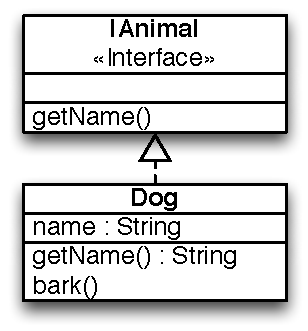
\includegraphics[width=4cm]{images/uml}
%     \caption{Sample UML Diagram}
%     \label{uml_example}
% \end{figure}

% \subsection{blubb 2}

% Avoid single subsections! Each ``parent'' has to have at least two ``childs''

% \section{bla 2}

\chapter{Introduction [1/2]}
	\section{Motivation, Why? -> ML needs this for Newton etc}
% \IMRADlabel{methods}
	\section{Overview}
		\subsection{Short summary of all implementation styles (i.e. CPS, Monad, tape, macro) [1/2]}
	\section{Details}
		\subsection{Example backpropagation by hand [1]}
		\subsection{Go through a real ML task (the implemented test) with "grad" as blackbox -> defines "goal" [1]}
% % \chapter{Implementation}

\chapter{Forward Mode Differentiation} \label{sec:forwardMode}

Forward mode differentiation by hand is straight forward and also translates well into code by sticking to our existing knowledge about symbolic differentiation (i.e. differentiation ``by hand''). Remember the sum and product rule
\begin{align*}
    \text{Sum rule}&: (f + g)' = f' + g' \\
    \text{Product rule}&: (f \cdot g)' = f \cdot g' + g' \cdot f \\
\intertext{and how to differentiate the variable and constants:}
    \text{Variable rule}&: \diff{x}{x} = 1 \\
    \text{Constant rule}&: \diff{c}{x} = 0\ (c \neq x) \\
\end{align*}
These four differentiation rules build the base for our forward mode implementations. Essentially we want to go through every expression recursively and replace it with its derivative.


\section{Code replacement with macros} \label{sec:macros}
If you take the last sentence literally you could now go the long and hard way (which we did), learn metaprogramming and implement it exactly by replacing expressions with their derivative by directly applying the aforementioned differentiation rules. This approach looks rather ugly at first sight but after ignoring the boilerplate (with the help of the comments on the right-hand side) one can see that it just boils down to recursive pattern matching of code which works pretty intuitively in Scala 3~\cite{maScala3}:
\begin{lstlisting}
def d(t: Expr[Term])(using Quotes): Expr[Term] = t match
    case '{ ($l: Term) + ($r: Term) } =>    // l + r
        '{ ${ d(l) } + ${ d(r) } }          // d(l) + d(r)
    case '{ ($l: Term) * ($r: Term) } =>    // l * r
        '{ $l * ${ d(r) } + ${ d(l) } * $r }// l * d(r) + d(l) * r
    case '{ X } => '{ 1 }                   // variable
    case '{ $v: V } => '{ 0 }               // constant
\end{lstlisting}
 Ignore all types of line 1 and just think of \lstinline{t} as a (sub-)term (or expression for that matter) of a mathematical function we want to differentiate by calling \lstinline{d}. Now take for example line 2. We match \lstinline{t} to be a sum of two (sub-)terms (named \lstinline{l} and \lstinline{r}). In line 3 we have to define how \lstinline{t} should be replaced to get the derivative. For that we use the sum rule and essentially return \lstinline{d(l) + d(r)} which recursively applies the differentiation operator. The main challenge here is to ignore all those braces, dollar signs and apostrophes which are essentially a necessary evil to write macros but lets us intuitively pattern match over \emph{type checked} code which is a really powerful tool. Line 4 and 5 do the same but use the product rule. Line 6 matches the term to be \lstinline{X} which denotes our variable and is differentiated to 1. Analogously if a value is of type \lstinline{V} like in line 7 it is a constant which differentiates to 0.

In fact, we would not even need macros and could just write our term with algebraic data types and recursively match them at runtime to implement this approach. This would reduce the boilerplate in comparison to this macro-implementation.


\section{Operator overloading with dual numbers}\label{sec:forwardDualNumbers}

Rewriting code that way has one problem. We loose the actual result of our formula and only get the derivative (or we would have to calculate both separately). Consider we have the following function:
\begin{lstlisting}
def f(x: Double): Double = 2 * x + x * x * x
\end{lstlisting}
By writing \lstinline{f(3)} we can now calculate the result. Our goal is to simultaneously calculate the result and derivative of each subexpression to ultimately accumulate it into the final result and derivative. For this, we could use a structure that consists of two values. Such a construct is called a "dual number" and consequently has two members, one representing the value of an expression and the other representing the derivative of that expression:
\begin{lstlisting}
case class Dual(v: Double, d: Double)
\end{lstlisting}
To implement operations on dual numbers we have to define the actual computation and additionally how to compute the derivative:
\begin{lstlisting}[caption={Dual number implementation}, label={lst:forwardDualNumber}]
case class Dual(v: Double, d: Double):
    def *(that: Dual) = Dual(
      this.v * that.v,
      this.v * that.d + this.d * that.v // product rule
    )
  
    def +(that: Dual) = Dual(
      this.v + that.v,
      this.d + that.d // sum rule
    )
\end{lstlisting}
For multiplication this means that we can just multiply to get the actual result (line 3) and have to apply the product rule in line 4 by accessing \lstinline{v} to get the actual value and \lstinline{d} to get the derivative of the child expressions \lstinline{this} and \lstinline{that}. Addition works analogously but uses the sum rule.  As we can see, this comes down to translating mathematic symbolic differentiation rules into code. How to define constants and the variable (i.e. x) also comes naturally from the differentiation rules as the variable differentiates to 1 and constants to 0:
\begin{lstlisting}
def variable(v: Double) = Dual(v, 1)
def const(v: Double) = Dual(v, 0)
\end{lstlisting}
Differentiation of a function $f$ at $x = 3$ could then look like this:
\begin{lstlisting}[caption={Differentiation of a dual number function}, label={lst:forwardDualNumberDiff}]
def differentiate(f: Dual => Dual)(x: Double): Double =
    val result: Dual = f(variable(x))
    result.d // result.v would be the actual result of f(x)

def f(x: Dual): Dual = const(2) * x + x * x * x

val derivative = differentiate(f)(3)
\end{lstlisting}
The \lstinline{differentiate} function (line 1) essentially just applies a function to an argument for us (line 2) and then returns \lstinline{d} (i.e. the derivative) of the result (line 3).



\section{Match Types} \label{sec:matchTypes}
To explain the following approach we first have to look at match types which are essentially functions but at type level. Given a type, it uses patter-matching over that type to decide which type to return. It gets clear with the following example taken from the Scala 3 docs \cite{matchTypesScala3}:
\begin{lstlisting}
type Elem[X] = X match
    case String => Char
    case Array[t] => t
    case Iterable[t] => t
\end{lstlisting}
The match type \lstinline{Elem} has one argument \lstinline{X}. If \lstinline{X} is \lstinline{String} then it returns the type \lstinline{Char} (line 2). If \lstinline{X} is \lstinline{Array[t]} or \lstinline{Iterable[t]} it returns the generic type parameter of them, that is \lstinline{t}. In essence \lstinline{Elem} matches list-likes types and returns their element type. For example, it could be used like this:
\begin{lstlisting}
val i: Elem[Array[Int]] = 123
\end{lstlisting}
\lstinline{X} is in this case \lstinline{Array[Int]} and \lstinline{t} is therefore \lstinline{Int}. The type of \lstinline{i} ultimately reduces to \lstinline{Int}. By recursively matching types we can implement a differentiator match type \lstinline{D} purely at type level:
\begin{lstlisting}
type D[T <: Term] <: Term = T match
    case l * r => 
        l * D[r] + D[l] * r
    case l + r => 
        D[l] + D[r]
    case X => 
        V[1]
    case V[_] => 
        V[0]
\end{lstlisting}
\lstinline{D} itself and its argument \lstinline{T} are of type \lstinline{Term} which is just the super type of all of our expressions.
\lstinline{T} is a type but encodes a full calculation. Consider line 2 where we match \lstinline{T} to be \lstinline{l * r}. \lstinline{l} and \lstinline{r} are child \lstinline{Term}s (but are still types). In fact, the multiplication sign (\lstinline{*}) is  an infix type and not a method. It has two type parameters (in this case \lstinline{l} and \lstinline{r}) and is also a subtype of \lstinline{Term}:
\begin{lstlisting}
type *[L <: Term, R <: Term] <: Term
\end{lstlisting}
At this point you could ask yourself, which values those types can have. But we deliberately omit the runtime values of all types because the \emph{complete} differentiation is done at type-level in compile time. The exact values are more or less irrelevant for the implementation logic. A type fully encodes a function and should be seen as some kind of value for now.

In line 3 we apply the product rule by using the matched subexpressions \lstinline{l} and \lstinline{r} and recursively using \lstinline{D} on them. Addition works analogously but uses the sum rule.

Line 7 and 9 still look suspicious. What are integers doing as a type parameter? These are compile time value types which are now supported in Scala 3:
\begin{lstlisting}
type V[C <: Double | Int] <: Term
\end{lstlisting}
\lstinline{C} is a \lstinline{Double} or \lstinline{Int} singleton value type. By using \lstinline{scala.compiletime.constValue[C]} we can extract the singleton value from a singleton type. With this we can encode (integer) numbers fully at type-level and even calculate with them, also at type-level in compile time. Using this and our differentiation rules for the variable we can match the variable (which is the type \lstinline{X}) in line 6 and return a type which encodes the number 1. We do the same for constants where we match any constant (denoted by ``\_'') and differentiate it to 0.

If we combine all functionalities described above we gain the possibility to define a function and produce its derivative entirely at type level:
\begin{lstlisting}
type F = X * X
type DF = D[F] // -> X * D[X] + D[X] * X -> X * V[1] + V[1] * X
// the "symbolic" differentiation is already completed here (at compile time)

// the following is necessary to compute an actual result from the derivative (at runtime)
val df: DF = initFromType[DF] 
val result: Double = df(3)
\end{lstlisting}
The type \lstinline{F} (line 1) is the function we want to differentiate with respect to \lstinline{X}. As mentioned before it does \emph{not} need a value. We use our match type \lstinline{D} to produce the new type \lstinline{DF} which is equivalent to \lstinline{X * V[1] + V[1] * X}. That is, because it matches \lstinline{F} to be multiplication and uses the product rule. At this point the differentiation is completed and \lstinline{DF} fully represents the differentiated function.

Unfortunately computing a result at type level is impossible because we want to support decimal numbers. Type level calculation with integers on the other hand would be very possible and is included in Scala 3. To allow decimals we have to use a function \lstinline{initFromType} which recursively matches the provided type and constructs a function value which computes the result later at runtime. Essentially this means that we still have to fall back to actual values at runtime if we want usable results from our implementation and ca not pull through a full implementation at type-level and in compile time.

Additionally, we had a major problems concerning compilation time. Multiple chained multiplications took minutes to compile. At first, we blamed our implementation because we shifted (almost) all of our logic into compile time. An update of the Scala compiler to the newest version (3.0.2 as of now) solved that problem. Compilation time now takes no longer than usual compilations.

\chapter{Reverse mode differentiation}\label{sec:reverseMode}

In contrast to forward mode differentiation which benefits highly from our intuition, reverse mode is not straight forward to implement and we even have to work constantly against our intuition.

At first let us introduce our running example function, called $y$:
\newcommand{\yExampleDiff}{
    \begin{alignat*}{2}
        y & = x_1 &  & + x_1 x_2 \\
          & = w_1 &  & + w_1 w_2 \\
          & = w_1    &  & + w_3       \\
          & =        &  & w_4
    \end{alignat*}
}
\yExampleDiff
We gave every possible subexpression a name $w_i$:
\begin{align*}
    w_1 &\coloneqq x_1 \\
    w_2 &\coloneqq x_2 \\
    w_3 &\coloneqq w_1 w_2 \\
    w_4 &\coloneqq w_1 + w_3 \\
\end{align*}
Note that the outermost expression has the largest index and the innermost expressions have the smallest indices. Order of indices at the same level do not matter. Also notice that each occurrence of a $x_i$ gets the same name as can be seen with $x_1$ which both got the name $w_1$. Other expressions which do share the same structure and are therefore equal but are not exactly a $x_i$ would \emph{not} have shared names. This is an important detail for later but does not concern us for now.

For our purpose each expression is either an operation acting on subexpressions (e.g.\ multiplication or addition) or a value (constant or variable). This can be conveniently visualized as an expression tree with operations as nodes and values as leaves. Both occurrences of $w_1$ have to have separate nodes to visualize our (later introduced) implementations better:

\begin{minipage}[c]{0.5\textwidth}
    \begin{alignat*}{2}
        & =        &  & w_4 \\
        \\
        & = w_1    &  & + w_3       \\
        \\
        & = w_1 &  & + w_1 w_2 \\
        \\
        y & = x_1 &  & + x_1 x_2 \\
    \end{alignat*}
\end{minipage}%%
\begin{minipage}[c]{0.5\textwidth}
    % https://tikzcd.yichuanshen.de/#N4Igdg9gJgpgziAXAbVABwnAlgFyxMJZABgBoAmAXVJADcBDAGwFcYkQAdDuZgIzhz0AxgGtgAdwD6ARgAEXLrIAeMgL4hVpdJlz5CKchWp0mrdlx79BoiZPLyFyu+s3bseAkWmlpxhizZETm4+AWExKQBmB0UAKhctEAx3PSJInz9TQODLMJspABYYjgdsMAS3XU8DUmJMgPMQq3DbAFZi2QBqCqSdD31kdKoafzMgi1DrCJkOlWkXYxgoAHN4IlAAMwAnCABbJEMQHAgkbxAACxh6KHZIMDYaQSxGW4I2VxBtvYPHk8QyC5XG5BO4PEC8GBgYEAuDnLAbHBIYgfL77RAFX4-QHXV73DSJVFIDFHP7pbHA8BvfGbHZosnHJCtGiXHEgqmqSiqIA
%    \begin{tikzcd}
%        &                                                             & \substack{w_5 \\ +} \arrow[ld, no head] \arrow[rd, no head] &                                           \\
%        & \substack{w_3 \\ *} \arrow[rd, no head] \arrow[ld, no head] &                                                             & \substack{w_4 \\ \sin} \arrow[d, no head] \\
%    \substack{w_1 \\ x_1} &                                                             & \substack{w_2 \\ x_2}                                       & \substack{w_1 \\ x_1}
%    \end{tikzcd}


    % https://tikzcd.yichuanshen.de/#N4Igdg9gJgpgziAXAbVABwnAlgFyxMJZABgBoAmAXVJADcBDAGwFcYkQB3AfQEYQBfUuky58hFOQrU6TVu27kBQkBmx4CRHqR7SGLNohAAdI3GYAjODnoBjANbBuAZgAEJky4BU-JcLViiJ21dWQNjUwsrWwduABY3dwTsMB9BP1ENCVJiEP12EzNLa3tHLgBWBI8AalTlVQzxZCCqGj05Q24+NJURdUagp1z2kAAPXl8e-0zkSUHW0PYxxW76vqIyOZk8wzGu6RgoAHN4IlAAMwAnCABbJEkQHAgkLRAACxh6KHZIMDYaaywjG+BDY3UuNzu-yeiDIbw+X0MPz+IHMMDACNhcFeWDOOCQxDBV1uiFiUMhcM+wN+E3BxNJD2hQQpCPAIJpRKQTMeSDKNHelMRbMJEMQvIZSAAbHz4VTQcpac8yYgAOzSgWs6nC4mw7mIAAcapZSIElH4QA
%    \begin{tikzcd}
%        &                                                             & \substack{w_5 \\ +} \arrow[ld, no head] \arrow[rd, no head] &                                           \\
%        & \substack{w_3 \\ *} \arrow[rd, no head] \arrow[ld, no head] &                                                             & \substack{w_4 \\ \sin} \arrow[d, no head] \\
%        w_1 \arrow[d, no head] &                                                             & w_2 \arrow[d, no head]                                      & w_1 \arrow[d, no head]                    \\
%        x_1                    &                                                             & x_2                                                         & x_1
%    \end{tikzcd}


    % https://tikzcd.yichuanshen.de/#N4Igdg9gJgpgziAXAbVABwnAlgFyxMJZABgBoBGAXVJADcBDAGwFcYkQB3AfXJAF9S6TLnyEUAJgrU6TVuwA68uMwBGcHPQDGAa2DcAzAAJFiwwCo+-QSAzY8BIuVLFpDFm0QhFytRp16uABZjE0MAaksBITtRIjJ9V1kPEAAPHitokQcUJ3FE93ZuXiibYXsxZH1SPJo3OU9ucQzSmOzkJwTapPY04utbLIqqzpkCzzSmvmkYKABzeCJQADMAJwgAWyRJEBwIJDIQAAsYeih2SDA2EtWNrZpdpCcjk7PPC6vrG83EJ4fEQJox1O5wIH2Wa2+vz2iAArICXiDLs0vkgATtoQA2eHAt6g5EQpBw9FIADs2Ne4Dx1wJiAOfyqzxxlKRUz4QA
    \begin{tikzcd}
        & \substack{w_4 \\ +} \arrow[ld, no head] \arrow[rd, no head] &                                                             &                        \\
        w_1 \arrow[dd, no head] &                                                             & \substack{w_3 \\ *} \arrow[ld, no head] \arrow[rd, no head] &                        \\
        & w_1 \arrow[d, no head]                                      &                                                             & w_2 \arrow[d, no head] \\
        x_1                     & x_1                                                         &                                                             & x_2
    \end{tikzcd}
\end{minipage}



\newcommand{\overw}[1]{\overline{w}_{#1}}
\newcommand{\diffyw}[1]{\diff{y}{w_{#1}}}
Forward and reverse mode differentiation are built on two different main formulas of concern:
\\
\begin{minipage}[c]{0.5\textwidth}
    \begin{equation*}
        \text{Derivative:}\ \dot w_i \coloneqq \diff{w_i}{x}
    \end{equation*}
\end{minipage}%
\begin{minipage}[c]{0.5\textwidth}
    \begin{equation*}
       \text{Adjoint:}\ \overw{i} \coloneqq \diffyw{i}
    \end{equation*}
\end{minipage}
\\ \\
In forward mode we compute the derivative from small $i$ to largest, i.e.\ from the leaves to the root of the tree. For example if $\dot w_1 = \dot x_1$ and $\dot w_2 = \dot x_2$ are given we can calculate (by using the product rule)
\[ \dot w_3 = w_1 \dot w_2 + \dot w_1 w_2. \]
With that we can then find $\dot w_4$. Note that as stated above we need to know the initial value of $\dot x_1$ and $\dot x_2$. If we had one single variable we would set it to $\dot x = \diff{x}{x} = 1$ and calculate our result. But as we have two variables we have to do two passes through the whole calculation, one with $\dot x_1 = 1, \dot x_2 = 0$ and one with $\dot x_1 = 0, \dot x_2 = 1$. Reverse mode does not have to do this. It only has to do one pass to calculate the same result which is the whole motivation to do reverse mode instead of forward mode. In fact for a function $f: \R^n \to \R^m$ forward mode has to do $n$ passes and reverse mode has to do $m$ passes through the whole function. Usually in machine learning tasks you have functions with $n >\! \!> m$ which are also very complex. You certainly want to do as least passes as possible.

For reverse mode we have to shift our focus from $\dot w_i$ to another main expression of concern, namely
\[ \overw{i} \coloneqq \diffyw{i} \]
also called the adjoint of $w_i$. Instead of calculating the derivative of a subexpression $w_i$ with respect to $x$ it expresses the derivative of $y$ with respect to a particular subexpression $w_i$ of $y$. Why this expression concerns us now gets clear after looking at the corresponding usage of the chain rule which both differentiation styles are based on. A quick reminder on the general definition of the chain rule:
\[ \diff{y}{x} = \diff{y}{z}\diff{z}{x} \]
Forward mode replaces all occurrences of $\dot w_i$ by using the chain rule which is the reason why that expression concerned us previously. The chain rule for backward mode is instead used to replace each occurrence of $\overw{i}$ recursively:
\newcommand{\diffw}[2]{\diff{w_{#1}}{w_{#2}}}
\[ \diff{y}{x} = \diffyw{1}\diff{w_1}{x} = \bigg(\diffyw{2}\diffw{2}{1}\bigg)\diff{w_1}{x} = \bigg(\bigg(\diffyw{3}\diffw{3}{2}\bigg)\diffw{2}{1}\bigg)\diff{w_1}{x} = \dots \]
On first sight it might look like we traverse from $i = 1$ to $5$. However as one calculates the expression in the innermost parentheses first one can easily see that the iteration actually goes from large to small index (i.e.\ root to leaves) opposed to forward mode.

This usage of the chain rule essentially dictates how we compute the reverse mode derivative. Our job is to calculate all $\overw{i}$ by applying the chain rule recursively until we have rewritten it into an expression including trivial subexpressions or $\overw{j}$ with $j > i$ (i.e.\ ancestor adjoints) which we would have already computed at that point. We use the same $y$ as above and calculate the adjoints of subexpressions $w_4$ to $w_2$ by applying the chain rule which constantly introduce parent expressions into the formula:
\yExampleDiff
\begin{align*}
    \overw{4}   & = \diffyw{4} = 1                                                                                                           \\
    \overw{3}   & = \diffyw{3} = \diffyw{4}\diffw{4}{3} = \overw{4}\diffw{4}{3} = 1                                                          \\
    \overw{2}   & = \diffyw{2} = \diffyw{4}\diffw{4}{2} = \diffyw{4}\diffw{4}{3}\diffw{3}{2} = \overw{4}\diffw{4}{3}\diffw{3}{2} = \overw{3}\diffw{3}{2} = w_1       \\
    \intertext{These were straight forward after recognizing the general pattern. Calculating $\overw{1}$ it not as straight forward:}
    \overw{1}^a & = \diffyw{1} = \diffyw{4}\diffw{4}{1} = \overw{4}\diffw{4}{1} = 1 \\
    \overw{1}^b & = \diffyw{1} = \diffyw{4}\diffw{4}{1} = \diffyw{4}\diffw{4}{3}\diffw{3}{1} = \overw{4}\diffw{4}{3}\diffw{3}{1} = \overw{3}\diffw{3}{1} = w_2       \\
    \overw{1}   & = \overw{1}^a + \overw{1}^b
\end{align*}
We had to realise that $w_1$ appears in two ``calculation branches'' and had to handle them separately. Lastly these partial adjoints (i.e. $\overw{1}^a$ and $\overw{1}^b$) of all branches then have to be summed (implying that if $w_1$ would occur $n$ times we had to sum $n$ results) into the full adjoint $\overw{1}$.

After some consideration and breaking down every step this process is not very complicated. This is true for a human who can overlook the whole expression including all its subexpressions. A program on the other hand often only has a limited view of the whole expression. Consider this translation of our example into code:
\begin{lstlisting}
def w3 = w1 * w2
def y = w1 + w3 // w4
\end{lstlisting}
At definition time of \lstinline{w3} we do not have enough information to calculate a full andjoint because only after adding all context with the definition of \lstinline{y} we know all branches where \lstinline{w1} occurs. In fact \lstinline{y} could also be just another subexpression of a bigger calculation. Usually when evaluating expressions you can start evaluating the innermost subexpression and use its result to evaluate its containing expression as we did for forward mode differentiation. This had the advantage that we could calculate the normal result values and the derivative of each subexpression simultaneously. Unfortunately this is not possible for reverse mode and directly using dual numbers as is does not suffice. We have to start with the top expression $w_4$ and have to work our way down to (all occurrences of) $w_1$ (and $w_2$). This is very unnatural to implement because the information flows in reverse order. On top of that when iterating from outer to inner expression we can no longer calculate the normal result. Naturally at some point we have to calculate these values too. The only option we have is to do a full \emph{forward pass} (inner to outer) to calculate the result values and another full \emph{backward pass} (outer to inner) to calculate the (partial) adjoints of every subexpression (also see \reffig{fig:informationFlow}). Fortunately the forward pass is trivial as it only has to calculate arithmetic results in usual recursive order.

\begin{center}
    % https://tikzcd.yichuanshen.de/#N4Igdg9gJgpgziAXAbVABwnAlgFyxMJZARgBoAmAXVJADcBDAGwFcYkQAdDuZgIzhz0AxgGtgAdwD6xAARcuMgB7SAviBWl0mXPkIoAzBWp0mrdlx79BoiZPJz5Su2o1bseAkXKlixhizZETm4+AWExKX0HBQAqF00QDHddIgAWHz9TQODLMJspVOiOB2wweLcdTwNSAAZMgPMQq3DbAFYimQBqcsTtDz1kdKoafzMgi1DrCOkO5WIepMqB1qMRrPZ1BMX+ohW6tYbxjhwYRRxgACcYWhgLuBgZAFtoGAW+lJQa1ZNDkE2KnafWr1MbBE5nYAAMwgF3E9AuUCeLxcxhgUAA5vAiKBIRcII8kN4QDgIEgyCAABYwehQdiQMBsGiCLCMOkENiuEC4-GEpmkxBfSnU2lBemMkC8GBgEWCuAUrCQnBIGqc7kExDpYn8olUmlshn-Ll49WaklIQxCvWi9mGtXmvlIFaWkXgG2q41IABsDsQAHYaHKFUrEABaImjbITZo2Ljg87Q2HwqAqDqx07nND0OBwFPyYppiFCfFoZgnHOp47p4ARnNqJn0Fn6jkJO1+n3ekCBxVIEPkiONXJTYAF85XG53V4VuPATPZ3OOEfAIuPEtl+cKRc0gBWECwYBwtdtHsQAA4fQBOGiMeiSxgABXeVRAFyw6IpSoD8u7AoOoKjeTERdl1XeB13zSsIRrMCHGnehpWgxdYBfBg8BuQ8VEoFQgA
%\begin{tikzcd}
%    \text{forward mode}                                                                               &                       &                                                             & \substack{w_5 \\ +} \arrow[ld, no head] \arrow[rd, no head] &                                           & \text{reverse mode} \arrow[dd, "\substack{\text{reverse} \\ \text{pass} \\ \text{computes} \\ \text{adjoints}}", shift left] \\
%                                                                                                      &                       & \substack{w_3 \\ *} \arrow[rd, no head] \arrow[ld, no head] &                                                             & \substack{w_4 \\ \sin} \arrow[d, no head] &                                                                                                                              \\
%    {} \arrow[uu, "\substack{\text{computes} \\ \text{values} \\ \text{and} \\ \text{derivatives}}"'] & \substack{w_1 \\ x_1} &                                                             & \substack{w_2 \\ x_2}                                       & \substack{w_1 \\ x_1}                     & {} \arrow[uu, "\substack{\text{forward} \\ \text{pass} \\ \text{computes} \\ \text{values}}", shift left=2]
%    \end{tikzcd}
%

% https://tikzcd.yichuanshen.de/#N4Igdg9gJgpgziAXAbVABwnAlgFyxMJZAZgBoBGAXVJADcBDAGwFcYkQAdDuZgIzhz0AxgGtgAdwD6xAARcuMgFQBfEMtLpMufIRQAmUgAZqdJq3Zce-QaImSALHPkyA1KvWbseAkXuk9JgwsbIic3HwCwmJSek4KAB6Seu4aIBheOkQArP6BZiEgaqnp2j4oOcY0QeahXDgw8TjAAE4wtDDNcDAyALbQMCmepbrIhrlV+exFQ94jY5WmwRYc9Y3AAGYQzeL0zVC9-YNpWrNE5BR5S7Xh1lF25HEcMonkRyWn+uOLNWFWkbZSB7yJ4vdwmGBQADm8CIoHWzQgPSQ5xAOAgSDGIAAFjB6FB2JAwGwPCB4YiMTQ0UgDNjcfjQoTiakyUjEGRUejEH4QHAsVh1jgkABaGnVAqWCI2MR1BpNTbbXZQZSPJyrJpoehwODK4Gq2XAISItDMeralUytZi7WqSn0LCMAkEJlwhGs7lUtk0Xn8wWIIUosXLP5S4AWpqtdqdAbmlb6jVanXOMMGo0m+CJhTJvEAKwgWDAOGt01JrqQOQ5SAAbDRGPReDBGAAFE6ZULNLCQrGCr18gUU77im7-aWxtaGnrG00Zp7Jq3TvVrehgJUxtXAWDthh4dpFkks5GUzkAdhoOLxjqJxf3iExHoAHKe6RfiZRlEA
    \begin{tikzcd}
        \text{forward mode}                                                                               &                       & \substack{w_4 \\ +} \arrow[rd, no head] \arrow[ld, no head] &                                                             &                       & \text{reverse mode} \arrow[dd, "\substack{\text{reverse} \\ \text{pass} \\ \text{computes} \\ \text{adjoints}}", shift left] \\
        & \substack{w_1 \\ x_1} &                                                             & \substack{w_3 \\ *} \arrow[rd, no head] \arrow[ld, no head] &                       &                                                                                                                              \\
        {} \arrow[uu, "\substack{\text{computes} \\ \text{values} \\ \text{and} \\ \text{derivatives}}"'] &                       & \substack{w_1 \\ x_1}                                       &                                                             & \substack{w_2 \\ x_2} & {} \arrow[uu, "\substack{\text{forward} \\ \text{pass} \\ \text{computes} \\ \text{values}}", shift left=2]
    \end{tikzcd}

    \captionsetup{type=figure}
    \caption{Information flow of forward and reverse mode}
    \label{fig:informationFlow}
\end{center}

The main takeaway from this extensive example is an important pattern which we will be utilizing to implement the reverse pass. The second last term of every calculation of $\overw{i}^z$ (i.e. the partial adjoint of the $z$-th occurrence of $w_i$) with $z \in \{a, b, ...\}$ has always the following pattern:
\newcommand{\defoverwiz}{\overw{i}^z = \overw{p}\diff{w_p}{w_i^z}}
\[ \defoverwiz \]
for some $p$. This $p$ (\emph{parent index}) is not at all random. $w_p$ is always the parent expression of that specific occurrence $w_i^z$ of $w_i$. We use the superscript to distinguish specific occurrences. We also could have written $y$ like (notice the added superscripts $a$ and $b$)
\begin{alignat*}{2}
    y & = x_1 &  & + x_1 x_2 \\
    & = w_1^a &  & + w_1^b w_2^a \\
    & = w_1^a    &  & + w_3^a       \\
    & =        &  & w_4^a
\end{alignat*}
to further emphasize distinct occurrences of expressions $w_i$. Usually we omit the superscript if that expression only occurs once. Actually $w_i$ can only occur multiple times (i.e.\ have a ``$b$'' superscript) if $w_i = x_i$, i.e\ the expression is one of our variables. In other words: Equal expressions are not counted as multiple occurrences and for that matter only $x_i$ count.

When boiling down
\[ \overw{i}^z = \overw{p}\diff{w_p}{w_i^z}\]
further we realise that we have to compute the derivative of the parent expression with respect to $w_i^z$. This is fortunately comparatively easy. A parent expression will always be an atomic operation (e.g. (*), (+), (-), $\sin$) and $w_i^z$ is always a direct argument. Because we usually know the derivative of each of our atomic operations, we can simply handle every case, e.g.\ if $w_p$ is a multiplication expression (and it has some right-hand side $w_k$) we can simply compute:
\[ \diff{w_p}{w_i^z} = \diff{(w_i^z \cdot w_k)}{w_i^z} = w_k \]
The remaining and main task is to find $\overw{p}$, the adjoint of the parent expression (i.e.\ the derivative of $y$ with respect to $w_p$). This is a recursive problem but unfortunately in reverse order because information flows from outer expression to inner which is the reason why this is called the reverse pass as already illustrated in \reffig{fig:informationFlow}. Solving this ``reversed flow of information'' to calculate $\overw{p}$ elegantly, efficiently or easily to reason about is the main goal of the following implementations.


\section{Using mutation} \label{sec:mutation}
\subsection{Continuation Passing Style (CPS)} \label{sec:cps}

Continuation is just an elaborate term for the frequently used callbacks (e.g.\ for frontend web development). Essentially you pass the ``rest of the calculation'' to the function instead of using its return value and manually applying the rest on that result. To make things clear consider chaining two arbitrary functions (with unspecified types \lstinline{A, B, C, D}) as usual on the left-hand side and an equal implementation but in CPS on the right-hand side:
\\
\begin{minipage}[c]{0.45\textwidth}
\begin{lstlisting}[caption={Ordinary chaining}, label={lst:ordinaryChaining}]
def first(x: A): B
def second(x: B): D

def chained(x: A): D =
  val firstResult: B = first(a)
  return second(firstResult)

val a: A = ???
val chainedResult: D =
  chained(a)
\end{lstlisting}
\end{minipage}%%
\begin{minipage}[c]{0.55\textwidth}
\begin{lstlisting}[caption={CPS chaining}, label={lst:cpsChaining}]
def first[R](x: A)(rest: B => R): R
def second[R](x: B)(rest: D => R): R

def chained[R](x: A)(ret: D => R): R =
  first(a) { (firstResult: B) =>
    second(firstResult) { ret }
  }
val a: A = ???
val chainedResult: D =
  chained(a) { identity }
\end{lstlisting}
\end{minipage}
\\
\\
On the left-hand side we first define two functions which have unspecified implementations. The types are the important part. \lstinline{first} takes \lstinline{A} and returns \lstinline{B}. \lstinline{B} is in turn the input type of \lstinline{second} which is important because this makes both functions chainable. \lstinline{chained} (line 4) calls \lstinline{first} (line 5) and passes its result to \lstinline{second} (line 6) which is essentially the definition of function chaining. Lines 8 to 10 just visualize how \lstinline{chained} is then used.

The right-hand side looks somewhat similar but has significant changes. Every function now has a second argument, i.e.\ the continuation which we usually call \lstinline{rest}. Notice that the \emph{input} type of \lstinline{rest} in \lstinline{first} of \reflst{lst:cpsChaining} is \lstinline{B}. This matches the \emph{result} type of \lstinline{first} in \reflst{lst:ordinaryChaining} (and analogously for \lstinline{D} and \lstinline{second}). Also note that we had to introduce type parameter \lstinline{R} to all functions. This is needed to support arbitrary \lstinline{rest} functions even if they do not return exactly \lstinline{D}. \lstinline{chained} works similarly but looks very different. We also call \lstinline{first} in line 5 but instead of creating a new named (constant) variable we have to pass a lambda where the parameter takes the role of the variable. After that we call \lstinline{second} and pass \lstinline{ret} as \lstinline{rest} which in this case has an equal semantic to the \lstinline{return} statement in line 6 of the left-hand side. In line 10 of \reflst{lst:cpsChaining} we pass \lstinline{identity} to \lstinline{chained} to mark the end of the calculation because it acts like a no-op. We could have passed another arbitrary operation instead, similarly to how we could have applied more arbitrary operations on \lstinline{chainedResult} in \reflst{lst:ordinaryChaining}. When following CPS strictly, every function takes a continuation and ordinary variables are never used. Lambdas with named parameters fulfill that role instead, as seen with \lstinline{firstResult} in line 5.

Using CPS which is an at first glance rather obscure feature we can implement reverse mode using dual numbers:
\begin{lstlisting}[mathescape=true, caption={Reverse mode CPS}, label={lst:cpsDual}]
case class Dual(x: Double, var adjoint: Double):
    def *(that: Dual)(k: Dual => Dual): Dual =
        // $ w_p $
        val localResult = Dual(this.x * that.x, 0)

        val globalResult = k(localResult)
        
        // $ i \in \{ \text{this}, \text{that} \} $
        def addPartialAdjoint(
            thisOrThat: Dual, 
            derivativeWrtThisOrThat: Double
        ): Unit =
            // $ \overw{i}^z = \overw{p} \diff{w_p}{w_i^z} $ 
            val partialAdjoint = 
                localResult.adjoint * derivativeWrtThisOrThat
            // $ \overw{i} \pluseq \overw{i}^z $
            thisOrThat.adjoint += partialAdjoint
        end addPartialAdjoint

        addPartialAdjoint(this, that.x) // $ i = \text{this} $
        addPartialAdjoint(that, this.x) // $ i = \text{that} $
        globalResult
    end *

    // Analogous to (*)
    def +(that: Dual)(k: Dual => Dual): Dual = ???
end Dual
\end{lstlisting}
Compared to forward dual numbers (\reflst{lst:forwardDualNumber}) we changed the name of the second member of \lstinline{Dual} to \lstinline{adjoint} to reflect the shift in focus from $\dot w_i$ to $\overw{i}$. The comments add translations from code expressions into their mathematic notation from \refsec{sec:reverseMode}. $w_p$ in line 13 signifies the parent expression, e.g. for multiplication we would write it like this:
\begin{align*}
    w_{\text{this}} &= \text{\lstinline{this}} \\
    w_{\text{that}} &= \text{\lstinline{that}} \\
    w_p &= w_{\text{this}} \cdot w_{\text{that}}
\end{align*}
The helper function \lstinline{addPartialAdjoint} (line 9) essentially just executes the mathematical expressions in lines 13 and 16 but generalizes over for which subexpression ($\overw{\text{this}}^z$ or $\overw{\text{that}}^z$) to compute the partial adjoint. The \lstinline{partialAdjoint} (line 14) is the adjoint of this specific occurrence of $ w_i^z $. Remember that we have to sum the partial adjoints of all occurrence to get the full adjoint. Exactly that happens in line 17 by mutating \lstinline{thisOrThat.adjoint}. Every expression is responsible to add the partial adjoints of their subexpressions. By translating every code piece into its corresponding mathematical notation, one can clearly see the close relationship between our implementation and the mathematical foundations of reverse mode differentiation seen in \refsec{sec:reverseMode}.

The main difference is line 6 where we call the continuation \lstinline{k}. It represents the rest of the computation as stated previously. In this context specifically, it represents all further operations that might use the passed \lstinline{localResult}. Note that those further operations are ancestors and not children or in other words they are outer and not inner operations. The first job of the continuation is to do an \emph{forward pass} through the rest of the operations. This is done by calculating the regular result (line 4) of the next operation and afterwards calling the next continuation. This recursive forward pass eventually finishes by calling a \lstinline{k} which does not call another continuation. At this point we found the recursion anchor and have built a stack of calls as usual with recursive algorithms. This built-up stack now naturally tears down in \emph{reverse order}. This is exactly our primary goal. We had to calculate the regular results in ``normal'' order (i.e. inner to outer expression) but the adjoint is naturally calculated in \emph{reverse order} (as seen in \reffig{fig:informationFlow}). The built-up stack is visualized in \reffig{fig:stack} for our running example. It tears down from top to bottom.
\begin{center}
    \tikzset{
		every node/.style={draw, text height=1.5ex},
		split/.style={rectangle split, rectangle split parts=#1,draw,
			rectangle split horizontal=false,rectangle split part align=base},
	}

    \begin{tikzpicture}[->, -{Latex}]
        \node[split=5] (a2) at (4,1) {\nodepart{one} $w_4\ (+)$ \nodepart{two} $w_1\ (x_1)$ \nodepart{three} $w_3 (*)$ \nodepart{four} $w_1 (x_1)$ \nodepart{five} $w_2 (x_2)$};
    \end{tikzpicture}

    \captionsetup{type=figure}
    \caption{Expression stack after the forward pass}
    \label{fig:stack}
\end{center}
From here on therefore the \emph{reverse pass} starts. On top of the stack now resides $w_4$. Lines 9 to 20 are executed to update the adjoint of its subexpressions ($w_1$ and $w_3$). After that, $w_1$ and then $w_3$ and its whole expression tree on the stack is handled. As you can see, after doing the forward pass by abusing continuations we now iterate through each expression in the same order as we would do when doing reverse differentiation by hand. Essentially we have linearized the expression tree to make the reverse pass and therefore adjoint accumulation easier. We use some kind of linearization in almost every reverse mode implementation.

In the end we define a \lstinline{differentiate} operator and call it:
\begin{lstlisting}[mathescape=true]
def differentiate(f: Dual => (Dual => Dual) => Dual)(x: Double): Double =
    val xDual = Dual(x, 0)

    // Use only side effects
    f(xDual) { topExpression => {
        // Manually set adjoint of top-most expression
        topExpression.adjoint = 1 // $\overline{y} = \diff{y}{y}$
        topExpression // $y$
    }
    }
    xDual.adjoint // $\overline{x} = \diff{y}{x}$
end differentiate

def f(x: Dual)(k: Dual => Dual): Dual =
    // 2 * x + x * x * x
    (Dual(2, 0) * x) { y1 =>
        (x * x) { y2 =>
            (y2 * x) { y3 =>
                (y1 + y3) { k }
            }
        }
    }
end f

val derivative: Double = differentiate(f)(3)
\end{lstlisting}
\lstinline{differentiate} in line 1 takes the function \lstinline{f} we want to differentiate as its first argument. Because we follow CPS \lstinline{f} has two inputs, first the input for \lstinline{x} of type \lstinline{Dual} and second the continuation of type \lstinline{(Dual => Dual)} which is called by \lstinline{f} itself after calculating its result. The result of the continuation is the final result of type \lstinline{Dual}. \lstinline{differentiate} also gets the \lstinline{Double} value passed at which we want to differentiate \lstinline{f}. In line 2 we create a \lstinline{Dual} from \lstinline{x}. Its initial adjoint has to be zero because its partial adjoints will get added to it by mutation later. The continuation passed to \lstinline{f} in line 5 is basically just an identity function to mark the top most expression and to act as the recursion anchor. We just have to additionally set the adjoint of the top expression to 1 because our program would not know which the top expression is. Another point to notice is that we do not directly use the result of \lstinline{f} and instead read the mutated adjoint of $x$ in line 11. This makes sense because \lstinline{f} returns the result of the \emph{top} expression. Its adjoint is trivially 1 (line 7) and therefore is not interesting while the adjoint of $x$ (line 11) is exactly the derivative of \lstinline{f}.

The biggest disadvantage of this CPS implementation is how one has to write the function \lstinline{f} compared to for example our forward mode dual number implementation in \reflst{lst:forwardDualNumberDiff}. Reading it is not impossible as one ``just'' has to read every line from right to left, that is on the right-hand side is the variable name (e.g. \lstinline{y1}) and on the left-hand side its ``value'' (e.g. \lstinline{2 * x}). We also have to give every subexpression a name which we would normally not need to and also often do not want to. Another problem is the deep nesting which occurs for more elaborate functions. A CPS function is therefore cumbersome to write and reading them needs some time getting used to. Those problems could be solved by using shift and reset operators which principally would make continuations implicit and would hide them completely from client code. Unfortunately there is currently no maintained implementation of them for Scala. Hence, we would like to refer to Fei Wang et al. \cite{lantern} and their implementation of reverse mode differentiation using shift and reset operators without further going into it here.

\subsection{Tape} \label{sec:tape}

The following implementation is very similar to CPS but instead of building a stack of calls implicitly by calling continuations we build that ``call stack'' manually. Remember that the only goal we achieved by using continuations was a two pass design which we used to do some operations (compute regular result) in normal order and some operations (compute adjoint) in reverse order through the expression tree. Another way to achieve this is to do the forward pass as usual but on the way additionally save all operations which have to be done in the reverse pass for later. When we have collected every operation we just execute them in ``reverse'' order:
\begin{lstlisting}[mathescape=true]
var tape: Unit => Unit = _ => ()

case class Dual(x: Double, var adjoint: Double):
    def *(that: Dual): Dual =
        val localResult = Dual(this.x * that.x, 0)

        def addPartialAdjoint(
            thisOrThat: Dual,
            derivativeWrtThisOrThat: Double
        ): Unit => Unit =
            _ =>
                val partialAdjoint = 
                    localResult.adjoint * derivativeWrtThisOrThat
                thisOrThat.adjoint += partialAdjoint
        end addPartialAdjoint

        tape = addPartialAdjoint(this, that.x) andThen tape
        tape = addPartialAdjoint(that, this.x) andThen tape

        localResult
    end *

    def +(that: Dual): Dual = ???
end Dual
\end{lstlisting}
Lines 5 to 14 which includes \lstinline{addPartialAdjoint} are in essence equal to the according lines in CPS and therefore we will just highlight the differences. We also omitted the mathematical translations. They are still important to get the connection to the mathematical foundations but for them refer to \reflst{lst:cpsDual} as they are very similar.

First thing to note is the altered return type of \lstinline{addPartialAdjoint} in line 10. It now returns a function which in turn is just used for its side effects (\lstinline{Unit => Unit} cannot take nor return anything meaningful). This means that when we call \lstinline{addPartialAdjoint} in line 16 and 17 the adjoint is \emph{not} directly updated opposed to CPS. Instead we prepend that ``operation'' (calculating and updating the adjoint of \lstinline{this} or \lstinline{that}) to \lstinline{tape}. We prepend (instead of appending) so that in the end we have a tape which executes each operation in reverse order of insertion. 

Our \lstinline{differentiate} function is again similar to CPS:
\begin{lstlisting}
def differentiate(f: Dual => Dual)(x: Double): Double =
    tape = _ => ()
    val xDual: Dual = Dual(x, 0)
    val topExpression = f(xDual)
    topExpression.adjoint = 1
    tape(())
    xDual.adjoint
end differentiate

def f(x: Dual): Dual =
    Dual(2, 0) * x + x * x * x

val derivative = differentiate(f)(3)
\end{lstlisting}
Because \lstinline{tape} is a global variable we have to remember to reset it for every differentiation (line 2). We then call \lstinline{f} in line 4 to do the forward pass and to populate the \lstinline{tape}. Similar to CPS we have to manually set the adjoint of the top expression to $1 = \diff{y}{y}$ (line 5). At this point no differentiation has been done yet. We have to call \lstinline{tape} to start it manually (as it takes a \lstinline{Unit} we have to pass its only inhabitant, namely ``\lstinline{()}''). The definition of \lstinline{f} (line 10 and 11) is possibly the most interesting change. We don't need any continuations and can omit variable names which makes it easier to read and write. 

To make the definition of \lstinline{f} even more regular we can define an implicit conversion which converts a constant into \lstinline{Dual} automatically. For this we use \lstinline{given} instances \cite{givensScala3} of \lstinline{Conversion} \cite{conversionsScala3} which were introduced in Scala 3. They specifically describe the intent to convert a value. Previously \lstinline{implicit} methods were used for this but their semantics were overloaded and for example have also been used to define extension methods. The first \lstinline{given} instance (line 1) is not needed for this example but is included for completeness if one uses decimal numbers:
\begin{lstlisting}
given Conversion[Double, Dual] = Dual(_, 0)
given Conversion[Int, Dual] = Dual(_, 0)

def f(x: Dual): Dual =
    // 2 is implicitly converted into Dual(2, 0)
    2 * x + x * x * x
\end{lstlisting}

So far we have only done reverse mode differentiation for one variable. As mentioned previously reverse mode differentiation shines when having multiple input variables. Therefore it's apparent to make an example which supports that. Extending the tape implementation to take multiple variables is mostly trivial as we only have to change the \lstinline{differentiate} function:
\begin{lstlisting}
def differentiate(
    f: List[Dual] => Dual, 
    xs: List[Double]
): List[Double] =
    tape = _ => ()
    val xsDual: List[Dual] = xs map { Dual(_, 0) }
    f(xsDual).adjoint = 1
    tape(())
    xsDual map { _.adjoint }
end differentiate

def f(xs: List[Dual]): Dual =
    2 * xs(0) + xs(1) * xs(2) * xs(2)

val derivatives: List[Double] = differentiate(f, List(3.0, 5.0, 2.0))
\end{lstlisting}
We encode multiple variables as a single vector of type \lstinline{List[Dual]}. Because \lstinline{f} now takes a \lstinline{List[Dual]}, \lstinline{differentiate} has to reflect that by accepting a function \lstinline{List[Dual] => Dual} and a vector of values to differentiate \lstinline{f} at. In line 6 we extract the \lstinline{adjoint} of each variable which ultimately gives us a vector where every value is the derivative with respect to one variable. In other words we computed the gradient of \lstinline{f}. The main takeaway here is that we computed the derivative of multiple variables in one go without having to call \lstinline{differentiate} multiple times with different values. This is only possible with reverse mode and is its main advantage. Forward mode would have to do one full differentiation for each variable where all other variable are set to 0.

Extending other reverse mode implementations for multi-dimensional functions (in input or output) is done analogously. To allow better focus on the essential differences and keep the examples simple we mostly concentrate on single dimensional functions from here on.
\subsection{Monad CPS} \label{sec:monadCPS}

We already established that writing CPS-functions by hand is cumbersome and not easily readable. We do not want to write deeply nested lambdas only to represent simple arithmetic calculations. Optimally we want to write arithmetic functions without a syntactic constraint, for example like this:
\begin{lstlisting}
2 * x + x * x * x
\end{lstlisting}
Because this is not translatable into CPS easily, the next best thing would be a syntax which resembles common usage of Scala to utilize our inherent intuition instead of breaking it. We introduce a named value for every subexpression. This does not change any semantics but conveniently separates each subexpression into its own line and own syntactic construct:
\begin{lstlisting}
val y1 = x * 2
val y2 = x * x
val y3 = y2 * x
val y4 = y1 + y3
\end{lstlisting}
Admittedly introducing a mandatory value name for every subexpression is not as elegant as directly writing down the expression. But value definitions are so ubiquitous that writing and reading them is at least very intuitive. The syntax should therefore look similar to this. Notice that we have only ``defined'' how we would like our code to look like and have not solved our problem yet as continuations are nowhere to be found yet. However we are not as far away from CPS as one could think. Remember how every continuation also has a mandatory named parameter which represents the result of the last calculation. By introducing mandatory named value definitions we have a somewhat similar situation at hand. Our goal is now to automatically rewrite these imperative value definitions into a CPS construct where each \lstinline{val} is translated into a continuation parameter and each subexpression is nested into the continuation of the last one.

Turns out Scala's for-comprehensions, if used in a specific way, can do exactly that. We mainly make use of the fact that a for-comprehension (without any guards) is entirely desugared into calls of multiple nested \lstinline{flatMap}s and one concluding \lstinline{map} for the \lstinline{yield}. If we manage to implement those two methods for our dual numbers, which is essentially equivalent to implementing a monad, we can write a function like this:
\begin{lstlisting}
def f(x: Dual): DualMonad
    for
        y1 <- x * 2
        y2 <- x * x
        y3 <- y2 * x
        y4 <- y1 + y3
    yield y4    
\end{lstlisting}
\lstinline{f} now returns a \lstinline{Monad} which wraps a dual number. Except of changed syntax the code is essentially similar to the imperative code of the last listing. The compiler then desugars it into this:
\begin{lstlisting}[caption={Desugared for-comprehension}, label={lst:desugaredForComprehension}]
def f(x: Dual): DualMonad =
    (x * 2).flatMap { y1 =>
        (x * x).flatMap { y2 =>
            (y2 * x).flatMap { y3 =>
                (y1 + y3).map { y4 =>
                    y4
                }
            }
        }
    }
end f  
\end{lstlisting}
At this point it should get clear why we wanted to use for-comprehensions to abstract over CPS. The compiler does the hard work for us and almost exactly translates a for-comprehension into CPS. Implementing \lstinline{flatMap} and \lstinline{map} (and thereby a monad) is the last (and main) task. The remaining code structure matches our previous CPS implementation.

Let's first look at the desired general signature for \lstinline{flatMap} and \lstinline{map} of a general monad:
\begin{lstlisting}
trait Monad[A]:
    def flatMap[B](f: A => Monad[B]): Monad[B] = ???
    def map[B](f: A => B): Monad[B] = ???
\end{lstlisting}
\lstinline{A} represents the value we are wrapping with the monad and \lstinline{B} is an arbitrary new type (possibly same as \lstinline{A}) which the value of \lstinline{A} is converted to. Both methods return a new monad which now wraps \lstinline{B}. In essence both methods model the mutation of the wrapped value and allow for the value type to change. The difference lies in the function passed to them. While the passed function to \lstinline{flatMap} returns a monad, the passed function to \lstinline{map} only returns a new value and \lstinline{map} has to wrap \lstinline{B} itself to be ultimately able to return \lstinline{Monad[B]}. 

A monad defined like this is very versatile because all value types are parameterized. This is important when using advanced capabilities of monads and to understand the concept in itself. For our use case on the other hand this is clearly excessive and can be simplified. The only value type we work on is \lstinline{Dual} and therefore we can replace all occurrences of \lstinline{A} and \lstinline{B} with simply \lstinline{Dual}. \lstinline{DualMonad} can be simply interpreted like an alias for \lstinline{Monad[Dual]}. For our purposes this is enough and makes the code easier to read without sacrificing expressiveness:
\begin{lstlisting}
trait DualMonad:
    def flatMap(k: Dual => DualMonad): DualMonad = ???
    def map(k: Dual => Dual): DualMonad = ???
\end{lstlisting}
We also renamed the passed functions into \lstinline{k} because they clearly represent continuations like one can easily see when looking at the desugared for-comprehension in \reflst{lst:desugaredForComprehension}. Let's look at the full implementation of \lstinline{Dual} and how we could implement \lstinline{DualMonad}:
\begin{lstlisting}
case class Dual(x: Double, var adjoint: Double):
    thisDual =>
  
    def *(thatDual: Dual): DualMonad = new DualMonad {
      override def flatMap(k: Dual => DualMonad): DualMonad =
        val parent = Dual(thisDual.x * thatDual.x, 0)
        val result = k(parent)
        thisDual.adjoint += thatDual.x * parent.adjoint
        thatDual.adjoint += thisDual.x * parent.adjoint
        result
  
      override def map(k: Dual => Dual): DualMonad =
        def wrap(dual: Dual): DualMonad = dual * 1
        flatMap(k andThen wrap)
    }

    def +(r: Dual): DualMonad = ???
end Dual
\end{lstlisting}
First notice that we do not implement \lstinline{DualMonad} at top level and in fact only implement it ad hoc when calling an operation on \lstinline{Dual}s. We use this to override \lstinline{flatMap} with the main operation logic which was found directly as part of \lstinline{*} (or \lstinline{+}) in previous reverse mode implementations. Because multiplication and addition have different logic we implement them ad hoc. When inspecting \lstinline{flatMap} further we realize that it is almost equivalent to the code of \lstinline{*} from the CPS implementation in \reflst{lst:cpsDual}. We calculate the parent result (line 6), call the continuation k to build the ``call stack'' (line 7) and then use the reverse pass to update the adjoints of \lstinline{thisDual} and \lstinline{thatDual} using the adjoint of the parent expression (lines 8-9). Note that we appended -\lstinline{Dual} to the instance name in line 2 to prevent a name clash with identifier \lstinline{this} when we are inside the ad hoc definition of \lstinline{DualMonad}. The only but important difference is that we eventually return the \lstinline{DualMonad} we got from the continuation in line 7. Returning a \lstinline{DualMonad} allows us to chain multiple \lstinline{flatMap} calls together which in turn means chaining multiple operations just like with normal CPS.

The next method we override is \lstinline{map} (line 12). The important signature difference to \lstinline{flatMap} is that it gets a function which returns a \lstinline{Dual} directly instead of a wrapped \lstinline{DualMonad}. Usually this is used to allow a last operation directly on \lstinline{Dual} before ending the for-comprehension. In our case this is not needed because each of our operations on \lstinline{Dual} return \lstinline{DualMonad} and not \lstinline{Dual}. Because of this the only \lstinline{k} which can be passed is a function which returns its argument or another \lstinline{Dual} captured by its closure. Essentially our job is to wrap the result of \lstinline{k} into a monad without changing the semantics. Naively one would try to implement \lstinline{DualMonad} ad hoc as we did with \lstinline{flatMap}. One unfortunately quickly realizes that we would have to implement another \lstinline{DualMonad} in the nested \lstinline{map} which leads us into an infinite loop of implementations. A solution for this is to apply a trivial identity function like multiplying with 1 to wrap a \lstinline{Dual} into a \lstinline{DualMonad} (line 13). With the ability to wrap a \lstinline{Dual} we can directly use the already implemented \lstinline{flatMap}. We just pass \lstinline{k} to it but wrap \lstinline{k}'s result into a \lstinline{DualMonad} to conform to \lstinline{flatMap}'s signature.

We successfully implemented a Monad and now just need a \lstinline{differentiate} function which sets the adjoint of the top expression to 1 just like in previous implementations. Additionally it has to wrap the top expression into a \lstinline{DualMonad} manually by again using a no-op multiplication (line 11):
\begin{lstlisting}
given Conversion[Double, Dual] = Dual(_, 0)
given Conversion[Int, Dual] = Dual(_, 0)

def differentiate(
    f: Dual => (Dual => DualMonad) => DualMonad, 
    x: Double
): Double =
    val xDual = Dual(x, 0)
    f(xDual) { topExpression =>
        topExpression.adjoint = 1
        topExpression * 1
    }
    xDual.adjoint
end differentiate
\end{lstlisting}
Note that the expected function \lstinline{f} again has a second argument, the continuation (\lstinline{Dual => DualMonad}) which now returns a \lstinline{DualMonad}.
Finally, we can use a for-comprehension to define \lstinline{f} to ultimately let the compiler rewrite our code into a CPS-like structure which was our goal:
\begin{lstlisting}
def f(x: Dual)(k: Dual => DualMonad): DualMonad =
    for
        y1 <- x * 2
        y2 <- x * x
        y3 <- y2 * x
        y4 <- y1 + y3
        y5 <- k(y4)
    yield y5
end f

val derivative = differentiate(f, 3)
\end{lstlisting}


\subsection{Combined Monad and Tape} \label{sec:monadAndTape}

Using for-comprehensions made the inside of a function more readable but when defining \lstinline{f} we still needed a continuation \lstinline{k} as its second parameter. This is not only ugly but makes it very hard to compose multiple functions. Instead, we want a simple way to define two functions \lstinline{f} and \lstinline{g} without seeing continuations at all and make chaining them as easy as writing \lstinline{f andThen g} as we are used to in Scala. We try to solve this by coming back to our tape based approach and combining it with our monad based one.

At first, we need our tape where we save all adjoint updates which have to happen in reverse order. This is exactly same to our first tape based implementation:
\begin{lstlisting}
var tape: Unit => Unit = _ => {}
\end{lstlisting}

Now we get back to monads. Previously we implemented \lstinline{DualMonad} ad hoc to overcome the different requirements of multiplication and addition. Those differences can be abstracted over which leads to a much cleaner and more reusable design. Essentially what we need to abstract over is the result of an parent calculation and how to update the adjoints of the child expressions using the parent adjoint. Those are both realized as members of \lstinline{DualMonad} and are called \lstinline{parent} and \lstinline{adjointsUpdater} respectively (line 1):
\begin{lstlisting}[caption={Monad using tape}, label={lst:monadTape}]
class DualMonad(val parent: Dual, val adjointsUpdater: Dual => Unit):
    def flatMap(k: Dual => DualMonad): DualMonad =
        tape = ((_: Unit) => adjointsUpdater(parent)) andThen tape
        k(parent)

    def map(k: Dual => Dual): DualMonad =
        flatMap(k andThen wrap)
end DualMonad

def wrap(dual: Dual): DualMonad = DualMonad(dual, identity)
\end{lstlisting}
\lstinline{flatMap} prepends the adjoint update operation to the tape (line 3) which is exactly what we did for our first tape implementation and then calls the continuation (line 4). \lstinline{map} is very similar to our first monad approach as it also just uses \lstinline{flatMap} after wrapping the result of \lstinline{k} (line 7). The difference is that instead of doing an no-op operation on \lstinline{Dual} we wrap it manually by passing a no-op identity function as the \lstinline{adjointUpdater} in the \lstinline{wrap} function (line 10).

We have already done the hardest task and now only have to glue the pieces together:
\begin{lstlisting}
case class Dual(x: Double, var adjoint: Double):
    def *(that: Dual): DualMonad =
        def addPartialAdjoint(
            thisOrThat: Dual,
            derivativeWrtThisOrThat: Double,
            parentAdjoint: Double
        ): Unit =
            val partialAdjoint = parentAdjoint * derivativeWrtThisOrThat
            thisOrThat.adjoint += partialAdjoint
        end addPartialAdjoint

        DualMonad(
            this.x * that.x,
            parent =>
                addPartialAdjoint(this, that.x, parent.adjoint)
                addPartialAdjoint(that, this.x, parent.adjoint)
        )
    end *

    def +(r: Dual): DualMonad = ???
end Dual
\end{lstlisting}
\lstinline{addPartialAdjoint} (line 3) is equal to previous implementations. We pass the normal result (line 13) and as usual how to update the adjoints of \lstinline{this} and \lstinline{that} to the constructor of \lstinline{DualMonad} (lines 14 to 16).

The biggest and most important change comes in the signature of \lstinline{differentiate}. The expected function \lstinline{f} uses no continuation and just expects and returns a \lstinline{DualMonad} which is exactly what we wanted:
\begin{lstlisting}
def differentiate(f: DualMonad => DualMonad)(x: Double): Double =
    tape = _ => ()
    val xDualMonad = wrap(Dual(x, 0))
    f(xDualMonad).parent.adjoint = 1
    tape(())
    xDualMonad.parent.adjoint
\end{lstlisting}
The implementation of it on the other hand is nothing special. Again, we have to remember to reset the tape (line 2). After wrapping a \lstinline{Double} into a \lstinline{Dual} and then into a \lstinline{DualMonad} (line 3) we have to call \lstinline{f} with it to do the forward pass and fill the tape (line 4). After setting the adjoint of the top expression (also line 4) we can execute the tape (and start the reverse pass) (line 5) which sets the adjoint of our argument to \lstinline{f}.

Because the expected function gets a \lstinline{DualMonad} and also returns one we can now easily chain two functions using \lstinline{andThen} (line 18) and still use for-comprehensions:
\begin{lstlisting}
def f(xM: DualMonad): DualMonad =
    for
        x <- xM
        y1 <- x * 2
        y2 <- x * x
        y3 <- y2 * x
        y4 <- y1 + y3
    yield y4
end f

def g(xM: DualMonad): DualMonad =
    for
        x <- xM
        y <- x * x
    yield y
end g

val derivative = differentiate(f andThen g)(3)
\end{lstlisting}
Note that one can interpret the first lines of the for-comprehensions (lines 3 and 13) as ``unwrapping'' the monad back into a \lstinline{Dual}.

\section{Without mutation} \label{sec:noMutation}
%\subsection{Why no mutation?}

\subsection{Continuation Passing Style (CPS)} \label{sec:functionalCps}

To eliminate mutation we have to firstly detect where mutation even occurs. Looking at the implementation of mutable CPS (\reflst{lst:cpsDual}) we directly find the culprit in the first line. The second member of \lstinline{Dual}, namely \lstinline{adjoint}, is mutable. As a matter of fact that is the only mutable state we use and therefore we have to remove it. \lstinline{Dual} is no longer a dual number when we remove its second member so we rename it to just \lstinline{Num} accordingly. Simply changing \lstinline{adjoint} to a \lstinline{val} would not suffice because we cannot know the adjoint of a \lstinline{Dual} at creation time because the adjoint has to be \emph{accumulated} from multiple branches. Adding an accumulator which is recursively propagated is consequently the logical next step. For this step we have to remember the obvious but critical fact that the reverse pass is indeed \emph{reverse} and we want to propagate the accumulator from parent to children. This is opposed to usual recursive algorithms where each child passes the accumulator to its parent until it reaches the top expression. The top expression uses the full accumulator to produce the full result. To achieve the reversed recursive pass through all expressions we still abuse continuations to build a stack which is naturally traversed in reverse order. The remaining task is to propagate the accumulator correctly. Let us look at the finished code and work along it to understand how one could implement that:
\pagebreak
\begin{lstlisting}
type Adjoints = Map[Num, Double]
type Continuation = Num => Adjoints

class Num(val x: Double):
    def *(that: Num)(k: Continuation): Adjoints =
        val parent = Num(this.x * that.x)

        def addPartialAdjoint(
            thisOrThat: Num, 
            derivativeWrtThisOrThat: Double, 
            adjoints: Adjoints
        ): Adjoints =
            val partialAdjoint = 
                adjoints(parent) * derivativeWrtThisOrThat
            val newAdjointThisOrThat = 
                adjoints(thisOrThat) + partialAdjoint
            adjoints + (thisOrThat -> newAdjointThisOrThat)
        end addPartialAdjoint

        val adjointsWithParent = k(parent)
        val adjointsWithThis = 
            addPartialAdjoint(this, that.x, adjointsWithParent)
        val adjointsWithThat = 
            addPartialAdjoint(that, this.x, adjointsWithThis)
        adjointsWithThat
    end *

    def +(that: Num)(k: Continuation): Adjoint = ???
end Num
\end{lstlisting}
In line 1 and 2 we assign names to two important types so that we can reason more easily about this implementation. The accumulator we use is of type \lstinline{Adjoints} and maps each expression to its currently accumulated adjoint. \lstinline{Continuation} is exactly that, the continuation of our program as seen before but with one major change. In previous implementations continuations returned the actual calculated result hence the type \lstinline{Dual => Dual} (\reflst{lst:cpsDual}). This seems somewhat convenient at first but we ignored the final result anyway (and could have used \lstinline{Unit} instead). Remember that continuations represent the calculation of ancestor expressions and so is perfectly suited to pass the currently accumulated adjoints to its descendants. Therefore continuations now return \lstinline{Adjoints} instead of \lstinline{Num}. 

The helper function \lstinline{addPartialAdjoint} (line 8) is very similar to the mutable approach (\reflst{lst:cpsDual}) but because \lstinline{Adjoints} is immutable it has to take the current adjoints as a parameter (line 11) and return an updated version with the added partial adjoint for \lstinline{thisOrThat} (line 17). Line 13 just computes the current partial adjoint using the adjoint of the parent expression which is exactly what happened in the mutable CPS implementation. Line 15 to 17 essentially just add \lstinline{partialAdjoint} onto the current value in the \lstinline{adjoints} accumulator. This translates exactly to the \lstinline{+=} operation used in the mutable version (\reflst{lst:cpsDual}).

Line 20 calls the continuation to get the adjoint of the current parent (and all other accumulated ancestor adjoints, potentially including \lstinline{this} or \lstinline{that}). Remember that at this point the stack builds up and the following lines are executed from top expression to children expressions. \lstinline{addPartialAdjoint} is called twice very similar to the mutable approach (lines 21 to 24). The most important part here is to always pass the latest updated adjoints to the next call. In the end we effectively return all adjoints of all ancestors we got from \lstinline{k} and also the updated adjoints of \lstinline{this} and \lstinline{that}. After we return, the next descendant now gets those updated adjoints from its call to its \lstinline{k}.

Finally we just have to define the usual \lstinline{differentiate} function. Note that the expected \lstinline{f} again expects a continuation and instead of returning the actual result of the calculation it now returns \lstinline{Adjoints} which contains all accumulated adjoints (line 5). As always we have to manually set the adjoint of the top expression to 1. In this case this is done by initializing the \lstinline{Adjoints} map with the \lstinline{topExpression} as key and 1 as value (line 10). Setting the default value of the map to 0 (also line 10) is also important. Basically it initializes all adjoints of all expressions to 0 so that we can sum all partial adjoints without checking first if the key already exists in the map.
\begin{lstlisting}
given Conversion[Double, Num] = Num(_)
given Conversion[Int, Num] = Num(_)

def differentiate(
    f: Num => Continuation => Adjoints, 
    x: Double
): Double =
    val xNum = Num(x)
    val allAdjoints = f(xNum) { (topExpression: Num) =>
        Map(topExpression -> 1.0).withDefaultValue(0)
    }
    allAdjoints(xNum)

def f(x: Num)(k: Continuation): Adjoints =
    (2 * x) { y1 =>
        (x * x) { y2 =>
            (y2 * x) { y3 =>
                (y1 + y3) { k }
            }
        }
    }

val derivative = differentiate(f, 3)
\end{lstlisting}
\subsection{Monad} \label{sec:functionalMonad}

Next we want to take a look at our approach where we combined monad and tape and remove every mutation. Similar to CPS in the last section we have the mutable member \lstinline{adjoint} of \lstinline{Dual}. Our solution for it was a map which functions as an adjoint accumulator and replaces the \lstinline{adjoint} member of \lstinline{Dual}. This will prove to be useful also for this problem:
\begin{lstlisting}
type Adjoints = Map[Num, Double]
\end{lstlisting}

A completely new obstacle is the tape itself which is also mutable. To convert it into something immutable let us first reflect which purpose it served. Principally it is a recursively accumulated list of operations which have to be executed later. Nothing speaks against passing a growing function (instead of a map for example) as an accumulator of our recursive pass through a calculation. In our case these operations always specifically acted with and on adjoints of some \lstinline{Dual}. Alas, \lstinline{Dual} has no \lstinline{adjoint} member anymore (and therefore was renamed into \lstinline{Num}). Its replacement is \lstinline{Adjoints} which keeps track of adjoints of every \lstinline{Num}. Consequently our ``tape accumulator'' has to act on \lstinline{Adjoints}. More specifically it has to be of type \lstinline{Adjoints => Adjoints} because you update the current (passed) adjoints by adding each child's partial adjoint and returning a new updated instance of \lstinline{Adjoints}. Previously every \lstinline{DualMonad} had a member \lstinline{adjointsUpdater: Dual => Unit} which was prepended to the tape to ultimately collect every \lstinline{adjointsUpdater}. We could instead use the member \lstinline{adjointsUpdater} itself as an accumulator by changing its type. Previously \lstinline{adjointsUpdater} just signified how to update the adjoints of one subexpression. Only on the tape they were chained. Now we directly chain each \lstinline{adjointsUpdater} recursively on the fly and pass the chained \lstinline{adjointsUpdater} to the outer \lstinline{DualMonad}. Thus we are now skipping the tape entirely by moving it into an accumulator (line 3):
\begin{lstlisting}
class DualMonad(
    val parent: Num, 
    val adjointsUpdater: Adjoints => Adjoints
):
    def flatMap(k: Num => DualMonad): DualMonad =
        val outerResult = k(parent)
        DualMonad(
            outerResult.parent, 
            outerResult.adjointsUpdater andThen this.adjointsUpdater 
        )
    end flatMap

    def map(k: Num => Num): DualMonad =
        flatMap(k andThen wrap)
end DualMonad

def wrap(n: Num): DualMonad = DualMonad(n, identity)
\end{lstlisting}
\lstinline{map} (line 13) follows the same logic as before in \reflst{lst:monadTape}. In \lstinline{flatMap} we first call the continuation to get the adjoints (and the normal result) of all outer expressions (line 6). \lstinline{outerResult.adjointsUpdater} is then a tape-like construct which captures how to update all adjoints from the top expression up until the current expression. By appending \lstinline{this.adjointsUpdater} in line 9 the operations are sorted from outer to inner which is the correct order we want to iterate through for the reverse pass of reverse mode differentiation.

Implementing \lstinline{Num} is trivial and is very similar to previous implementations . We just have to remember to always use the updated adjoint map in line 25 and 26 because \lstinline{addPartialAdjoint} returns a fresh object instead of mutating the old one:
\begin{lstlisting}
class Num(val x: Double):
    def *(that: Num): DualMonad =
        val parent = Num(this.x * that.x)


        def addPartialAdjoint(
            thisOrThat: Num, 
            derivativeWrtThisOrThat: Double, 
            adjoints: Adjoints
        ): Adjoints =
            val partialAdjoint = 
                adjoints(parent) * derivativeWrtThisOrThat
            val newAdjointThisOrThat = 
                adjoints(thisOrThat) + partialAdjoint
            adjoints + (thisOrThat -> newAdjointThisOrThat)
        end addPartialAdjoint


        DualMonad(
            parent,
            adjoints =>
                val adjointsWithThis = 
                    addPartialAdjoint(this, that.x, adjoints)
                val adjointsWithThat = 
                    addPartialAdjoint(that, this.x, adjointsWithThis)
                adjointsWithThat
        )
    end *

    def +(that: Num): DualMonad = ???
end Num
\end{lstlisting}

As always we have to implement \lstinline{differentiate}:
\begin{lstlisting}
def differentiate(f: DualMonad => DualMonad)(x: Double): Double =
    val xM: DualMonad = wrap(Num(x))
    val topMonad = f(xM)
    val initialAdjoints =
        Map.empty
            .withDefaultValue(0.0)
            .updated(topMonad.parent, 1.0)
    topMonad.adjointsUpdater(initialAdjoints)(xM.parent)
end differentiate

def f(xM: DualMonad): DualMonad =
    for
        x <- xM
        y1 <- x * 2
        y2 <- x * x
        y3 <- y2 * x
        y4 <- y1 + y3
    yield y4
end f

def g(xM: DualMonad): DualMonad =
    for
        x <- xM
        y <- x * x
    yield y
end g

val derivative = differentiate(f andThen g)(3)
\end{lstlisting}
At first we wrap the input \lstinline{Double} into a \lstinline{DualMonad} (line 1). When executing \lstinline{f} in line 3 we do not get a meaningful result yet. We only have the monad of the top expression of the calculation. But this monad contains an \lstinline{adjointsUpdater} which accumulated all operations needed to update an \lstinline{Adjoints} map from scratch into our full result. We create our initial \lstinline{Adjoints} map with default value 0, and we set the top expression to 1 (lines 4 to 7) just like for CPS. Finally, we can call \lstinline{topMonad.adjointsUpdater} on our \lstinline{initialAdjoints} and ultimately get the adjoint of \lstinline{xM} (line 8)

As one can see we did not have to sacrifice much to reach an implementation without mutation. Writing and chaining functions (lines 11 to 28) are exactly the same to the previous monad implementation. The implementation itself is arguably better structured because we do not have to implement \lstinline{DualMonad} ad hoc for every operation. Removing mutation and the global tape variable should also make the code easier to reason about. We also prevented at least one potential bug source because one had to remember to reset the tape for every calculation which is not a problem anymore. Furthermore, we could also argue that parallel execution using a global tape could lead to a multitude of problems which we wo not cover in more detail.
\subsection{Combinatory Homomorphic Automatic Differentiation (CHAD)} \label{sec:chad}

Until now we relied on a map to accumulate all adjoints of all expressions by mapping \lstinline{Num} to \lstinline{Double} to get rid of mutation. From a functional programming standpoint this is still a compromise. We mapped specific instances of \lstinline{Num} which means we have to generate an unique ID for every object to get a functioning map. In contrast imagine we would build our map by strictly comparing values (i.e. instances of \lstinline{Num} with the same numeric value are treated as indistinguishable). Sub-expressions of our calculation with the same result value would share one adjoint which is clearly flawed. To have a purely functional implementation we have to get rid of instance comparison which means to drop the map. We also take one step back from monads and return to dual numbers:
\begin{lstlisting}
case class Dual(v: Double, variableAdjoint: Double => Double):
    def *(that: Dual): Dual =
        def variableAdjointBothSides(
            partialAdjointThis: Double, 
            partialAdjointThat: Double
        ) =
            this.variableAdjoint(partialAdjointThis) 
                + that.variableAdjoint(partialAdjointThat)

        def partialAdjointThis(parentAdjoint: Double) = 
            parentAdjoint * that.v
            
        def partialAdjointThat(parentAdjoint: Double) = 
            parentAdjoint * this.v

        Dual(
            this.v * that.v,
            parentAdjoint =>
                variableAdjointBothSides(
                    partialAdjointThis(parentAdjoint), 
                    partialAdjointThat(parentAdjoint)
                )
        )
    end *

    def +(that: Dual): Dual = ???
\end{lstlisting}
First thing to notice is that \lstinline{Dual} now has a member named \lstinline{variableAdjoint: Double => Double} (line 1). It calculates an adjoint using the parent adjoint like already familiar. But the important difference (and the reason for the prefix ``variable-'') is that it does \emph{not} compute the partial adjoint of the current expression. It instead accumulates the sum of all partial adjoints of our variable (i.e. x). It ignores all partial adjoints of expressions not including x. We don't need them anyway.

Lines 10 to 14 look very familiar because it just computes the partial adjoints of \lstinline{this} and \lstinline{that}. From line 15 on we create a new \lstinline{Dual} with a new \lstinline{variableAdjoint}.  We calculate both partial adjoints (lines 20 and 21) and then pass it to \lstinline{variableAdjointBothSides}. \lstinline{variableAdjointBothSides}'s job is to sum the partial adjoints of x from both branches but has to ensure that only relevant partial adjoints are included and for example constants are ignored. The function does in fact just sum both variable adjoints together (lines 7 and 8). So where do we ensure that only relevant partial adjoints are summed? The answer lies in how constants and the variable are instantiated/defined:
\begin{lstlisting}
def variable(v: Double): Dual = Dual(v, identity)
def const(v: Double): Dual = Dual(v, _ => 0.0)
\end{lstlisting}
The partial adjoint of x is just directly its partial adjoint without further ado. This translates to the variable having \lstinline{identity} as its variable adjoint function (line 1). The variable adjoint of constants are always zero (line 2). This makes sense because constants have no meaningful partial adjoint for our variable. Effectively when \lstinline{variableAdjointBothSides} calls \lstinline{this.variableAdjoint(partialAdjointThis)} and \lstinline{this} is the variable x then it evaluates to \lstinline{partialAdjointThis}. If \lstinline{this} is a constant the call evaluates to zero. If \lstinline{this} is neither (e.g. a multiplication expression) then the previous two rules are implicitly applied for all branches of that expression recursively. This, after some consideration, rather simple design is sufficient to implement reverse mode differentiation fully functionally and without building some kind of virtual stack/tape as we did previously.

Another advantage of this approach is its simplicity for the user:
\begin{lstlisting}
given Conversion[Double, Dual] = const(_)
given Conversion[Int, Dual] = const(_)

def f(xDouble: Double): Dual =
    val x: Dual = variable(xDouble)
    2 * x + x * x * x
end f

val derivative = f(3).variableAdjoint(1)
\end{lstlisting}
After declaring the variable explicitly (line 5) (and using given conversions (lines 1 and 2) for constants) we can write \lstinline{f} simply like a usual arithmetic expression in Scala (line 6). We don't even need a \lstinline{differentiate} function because we accumulate the correct adjoint of x on the fly while calculating the result of \lstinline{f}. In previous reverse mode implementations we called \lstinline{adjoint} on x to get its adjoint which makes sense from a mathematical standpoint because we are interested in the adjoint of our variable and nothing else. In this case however we have to call \lstinline{variableAdjoint} on the result of \lstinline{f}. Ultimately we obviously still get the adjoint of x but the semantics of \lstinline{variableAdjoint} are different (as the name suggests). It can be most easily interpreted as the sum of all partial adjoints of x contained in all branches of the current expression. Therefore, we must call it on the outermost expression to include all partial adjoints of x in our whole calculation.

\chapter{Implementation}
	\section{Forward mode [1]}
		\subsection{by operator overloading (including macros)}
		\subsection{Match type implementation (and bad performance). Explain type level calculations (Peano). Pro/Con [1]}

	\section{Backpropagation with mutation}
		\subsection{Tape [1/2]} %maybe first?
		\subsection{CPS}
			\subsection{Explain Continuations (without shift/reset) [1/2]}
			\subsection{Encode backward pass as continuation [1/2]}
		\subsection{MonadCPS}
			\subsection{ -- For-comprehensions (flatMap, map) [1/2]}
			\subsection{ -- First try: .map() "closes" monad [1/2] }
			\subsection{ -- Second try: Chaining of functions with global tape [1/2]}

	\section{Backpropagation without mutation (functional)}
		\subsection{Why functional? (state, multiple calculations, reasoning) [1/2]}
		\subsection{CPS, MonadCPS [1]}
		\subsection{Tape}
			\subsection{ -- First try: naive (val, var difference -> multiple updates) [1/2]}
			\subsection{ -- Second try: Every node has to be calculated once [1]}
		\subsection{Con: (speed, ...) [1]}

    \section{Macros? [2]}


% \IMRADlabel{results}
\chapter{Evaluation}
	\section{List all comparison metrics (Runtime, LOC, compile time) [1]}
	\section{Interpretation [1/2]}
\chapter{Related work}
	\section{lantern paper [1/2]}

% \IMRADlabel{discussion}
\chapter{Conclusion [1/2]}



% Pages: 15
\printbibliography

\end{document}
